% The main file for my thesis
% each \textbf{chapter} is included from this main file
\documentclass[11pt,a4paper]{uolthesis}
%\documentclass[11pt,a4paper]{article}
%\usepackage{alltt,float}
%\usepackage{lgrind}
%\usepackage{url}                    % for better handling of URL
\usepackage{lscape}                 % allow to use \begin{landscape}, which makes a page in landscape.
%\usepackage{subfigure}
\usepackage[T1]{fontenc}
\usepackage{mathrsfs}
\usepackage{graphicx}
%\usepackage{caption2}
%\usepackage{epstopdf}
%\usepackage{biblatex}[natbib]
%\usepackage{natbib}
%\usepackage[natbibapa]{apacite}
%\usepackage{natbib}
%\usepackage{biblatex}[natbib]
\usepackage{amsmath}
\usepackage{tikz}
\usepackage{pgfplots}
\usepackage{caption}
\usepackage{subcaption}
%\usepackage{pgfgantt}
\usepackage{multirow}
\usepackage{caption}
\usepackage{subcaption}
\usepackage{pgfplots}
\usepackage{tikz}
%\usepackage[maxnames=4,minnames=3,maxbibnames=99]{biblatex}
\usetikzlibrary{positioning}

\usetikzlibrary{shapes.arrows}

%\let\cite\shortcite

\newcommand{\citepos}[1]{\citeauthor{#1}'s \citeyearpar{#1}}
\newcommand{\citeposs}[1]{\citeauthor{#1}' \citeyearpar{#1}}
%\newcommand{\argmax}[1]{\underset{#1}{\operatorname{arg}\,\operatorname{max}}\;}
\DeclareMathOperator*{\argmax}{argmax}

%Modify the Figure Captionequ1-1:shannon
%\renewcommand{\figurename}{Fig.}
%set the figures captions
%\captionstyle{hang} \setcaptionwidth{13cm}
%**********************************************

% correct bad hyphenation here
\hyphenation{op-tical}
% use less hyphenation
\lesshyphenation
% or totally stop it
%\nohyphenation

% include them only, as I am currently working on them
%\includeonly{ch1/ch1}

% begin the main document
\begin{document}

% include the title pages, acknowledgements, and author's publications

\title{Stage Two Report:\\
A Statistical Language Model for the Generation of Figurative Language}

\author{Stephen McGregor}
\department{Department of Electronic Engineering} \college{Queen Mary, University of London}
\degree{Doctor of Philosophy} \degreemonth{September} \degreeyear{2015}

%% By default, the thesis will be copyrighted to MIT.  If you need to
%% copyright the thesis to yourself, just specify the `vi' documentstyle
%% option.  If for some reason you want to exactly specify the copyright
%% notice text, you can use the \copyrightnoticetext command.
%\copyrightnoticetext{\copyright ~University of London, 2006}

% The dedication info.
%\dedication{TO MY FAMILY}

% Make the titlepage based on the above information.  If you need something
% special and can't use the standard form, you can specify the exact text of
% the titlepage yourself.  Put it in a titlepage environment and leave blank
% lines where you want vertical space. The spaces will be adjusted to fill
% the entire page. The dotted lines for the signatures are made with the
% \signature command.

% Make the first title page
\maketitle

% make the dedication page
%\makededication

% Start to count page number from abstract page
\pagestyle{plain}%
\setcounter{page}{1}
\pagenumbering{roman} %

% The abstractpage environment sets up everything on the page except the
% text itself.
%
% You can either \input (*not* \include) your abstract file, or you can put
% the text of the abstract directly between the \begin{abstract} and
% \end{abstract} commands.
\begin{abstract}
%\input{abstract}
% abstract goes here
MIMO (Multiple Input Multiple Output) technology has been regarded as a practical approach to
increase the wireless channel capacity and reliability.

Abstract goes here...


\end{abstract}

% Acknowledgments
%
% You can either \input (*not* \include) your acknowledgments file, or you can put
% the text of the acknowledgments directly between the \begin{acknowledgments} and
% \end{acknowledgments} commands.
%\begin{acknowledgments}
%\input{acknowledgments}
%Acknowledgment goes here...

%\end{acknowledgments}


%\include{format}
% Generate table of contents and the list of figures, tables and abbreviations
\tableofcontents
% create the toc, lof, and lot, they are added into toc by tocbibind package
\tableofcontents   % Create Table of Contents
\listoffigures     % Create List of Figures%
\listoftables      % Create List of Tables%

%List of Abbreviations
\chapter*{List of Abbreviations}
  \addcontentsline{toc}{chapter}{List of Abbreviations}
\begin{tabular}{ll}
\\
3D & Three-Dimensional\\

3G & Third Generation\\

3GPP & Third Generation Partnership Project\\

4G & Fourth-Generation\\

A-GPS & Assisted-GPS\\

AOA & Angle of Arrival\\

AWGN & Additive White Gaussian Noise\\

BLAST & Bell Labs Layered Space Time\\

BT & Base Station\\

CA & Circular Array\\

CDF & Cumulative Distribution Function\\

DECT  &  Digital Enhanced Cordless Telecommunications\\

DF & Degradation Factor\\

DLR & German Aerospace Centre\\


DR & Dielectric Resonator\\

EU  & European Commission \\


EVD & Eigen Value Decomposition \\

GAC & Galileo Advanced Concept\\



\\
\end{tabular}


\begin{tabular}{ll}
\\

GJU & Galileo Joint Undertaking\\

GO & Geometrical Optics\\

GPS & Global Positioning System \\

GSM & Global System for Mobile Communications\\

GTD & Geometrical Theory of Diffraction\\

IEEE & Institute of Electrical and Electronics Engineers\\

IFA & Inverted-F Antenna\\

iid & independent and identically distributed\\

ILA & Inverted-L Antenna\\

IP & Internet Protocol\\

IST & Information Society Technologies\\

LTE & Long Term Evolution\\

MIMO & Multiple Input Multiple Output\\

MT & Mobile Terminal\\

NLOS & Non-line-of-sight\\

NMHA & Normal Mode Helix Antenna\\

OFDM & Orthogonal Frequency Division Multiplexing\\

PCS  & Personal Communication Services\\

PDA & Personal Digital Assistant\\

PDC & Personal Digital Communications\\

PIFA & Planar Inverted-F Antenna\\

QMUL & Queen Mary, University of London\\

RF & Radio Frequency\\

RHCP & Right Hand Circular Polarisation\\

RT & Ray Tracing\\

Rx & Receiver \\






\\
\end{tabular}

\begin{tabular}{ll}
\\

SBR & Shooting and Bouncing Ray\\

SC & Selection Combiner\\

SIMO & Single Input Multiple Output\\

SISO & Single Input Single Output\\

SNR & Signal-to-noise ratio\\

SVD & Singular Value Decomposition\\

Tx & Transmitter\\

ULA & Uniform Linear Array \\


UTD & Uniform Theory of Diffraction\\


UTD & Uniform Theory of Diffraction\\

WiMAX & Worldwide Interoperability for Microwave Access\\

WLAN & Wireless Local Area Network\\

WP & Work Package\\

XPR & Cross-polar ratio\\



\\
\end{tabular}


\newpage

% begin of main text
\setcounter{page}{1} %
\pagenumbering{arabic}
% enable the headers
\pagestyle{fancy}


%\setcounter{chapter}{-1}
%\setcounter{page}{1}
\pagenumbering{arabic}

\setcounter{chapter}{2}

% Start the main context
%\setcounter{page}{1}
\pagenumbering{arabic}

\chapter{Preamble: Stage 2 Report}
This document presents the state of my PhD research as I enter the third year of my studies at Queen Mary.  My research project will be introduced properly in Chapter 1.  This preliminary chapter serves simply to introduce this document, which I hope will serve as the kernel of a full dissertation.  The following sections will lay out the work accomplished to date, both in terms of publications and experiments, and will also project the work that lies ahead over the next 18 months.  The rest of this document will hopefully serve as a template for the final presentation of my PhD, both as an outline and as a guide for the work the remains to be done.  No section is even close to complete, and some, particularly later in the document, are essentially empty, as the bulk of evaluative work on this project is pending.

\section{Completed, Ongoing, and Future Publications}
I've published five conference papers to date, with a potential forthcoming journal publication currently undergoing a first round of revision.  \cite{McGregor2014} explores the relationship between computational creativity and intellectual property law, and, in so doing, drew out some of the inherent difficulties in evaluating the output of a symbol manipulating system in terms creativity.  Related theoretical work was presented in \cite{McGregorEA2014}, where we address the philosophically problematic relationship between cognition and mental representation from the perspective of the analysis of creativity.  An idea central to my PhD work emerges from these two early papers: in order for the behaviour of an agent to be perceived as creative, the agent must offer an observer at least the facsimile of some sort of system of internal representations that dynamically interact with each other and with the environment to produce artefacts.

\cite{McGregorEA2015} continues in a philosophical vein, raising questions about the emergence of the type of goal-directed behaviour that is often taken to be implicit in acts of creation.  Again with a thoroughly theoretical grounding, \cite{McGregorEA2015b} introduces an overview of some of the computational approaches that will be used to map between geometric representations of conceptual spaces by way of generating interesting new metaphors.  The idea of using the geometric properties of distributional semantic models to perform metaphoric mappings was also presented by me at a talk at ICLC this past summer, though the talk was accompanied by an abstract rather than a full paper, as seems to be the norm with theoretical linguistic conferences.  In a much more empirically oriented paper, \cite{AgresEA2015} outlines for the first time the methodology for building a high-dimensional statistical language model which can be used to project conceptual subspaces in a momentary, contextually informed way.  This practical work is pushed further in \cite{McGregorEA2015c}, with an in-depth description of the model and further experiments designed to reveal its ability to map from language to contextually nuanced conceptual spaces.

My plan for the months ahead, in terms of research and corresponding publication, is to expand the headway made in the work published thus far towards the completion of two general tasks with a well established history in the computational linguistic literature: taxonomy recapitulation and analogy completion.  The general approach to analogy completion has already been outlined in \cite{McGregorEA2015b}, and I think we're getting close to the point where the model will be ready to handle some of the existing test sets for this type of task.  In terms of the construction of lexical ontologies, this kind of process is even more immediately inherent in the work already presented in \cite{AgresEA2015,McGregorEA2015c}.  With regard to these two anticipated results, I envision targeting some of the major summertime computational linguistic conferences such as ACL and EMNLP with highly empirical articles, and imagine there would also be ample material for one or two subsequent journal articles pending strong results.

\section{Schedule for the Next 18 Months}
What has been accomplished so far is the design and implementation of a contextually sensitive distributional semantic language model.  Ongoing experiments are confirming the hypothesis that this model is good at returning clusters of words which can be mapped as conceptual constituents.  The way forward for using this model for constructing lexical ontologies (ie, taxonomies) seems fairly clear.  Early experiments comparing the geometries of word clusterings within different spaces suggests that the intuition that congruence should provide a mechanism for analogy completion have also returned fairly positive results.

Following on this continued investigation, I plan on spending some time considering ways in which the dimensional reduction process might be described in a more mathematically rigorous way---my hunch at the moment is that there might be a way to consider this aspect of the model's operation in terms of a Laplacian matrix or perhaps a Riemannian manifold, but I need to do considerably more research in this direction.  It would be nice to have a more mathematically rigorous way of describing the model.  For the time being this notion remains speculative, so I will not include it in the thesis outline that follows, but it would be a nice way of objectifying some of the work that's already been done and so in my opinion deserves further consideration.

The two well-defined targets for the months ahead, taxonomy recapitulation and analogy completion, each culminate in a conference paper deadline.  Some conceptual work remains to be done: the way that the model speculates about seed clusters for different sense of a hypernymic term is under development, and the mechanism for exploring the geometry of clusters within subspaces likewise requires further investigation.  These experimental exercises will lead on to the development of the model's metaphor generating facilities, which will serve as the basis for the ultimate demonstration of the strength of this project as a practical exposition of a theoretical stance on the nature of language.

\begin{figure}[t]
	\caption{Scheduling for the Final 18 Months}
	\scriptsize
	\begin{center}
		\begin{ganttchart}[vgrid={*{30}{white},*{1}{black,dotted},*{29}{white},*{1}{black,dotted},*{30}{white},*{1}{black,dotted},*{30}{white},*{1}{black,dotted},*{28}{white},*{1}{black,dotted},*{30}{white},*{1}{black,dotted},*{29}{white},*{1}{black,dotted},*{30}{white},*{1}{black,dotted},*{29}{white},*{1}{black,dotted},*{30}{white},*{1}{black,dotted},*{30}{white},*{1}{black,dotted},*{29}{white},*{1}{black,dotted}},hgrid,x unit=0.2mm,y unit chart=5mm,time slot format=isodate,link bulge=10,link tolerance=300,group peaks width=10,group peaks tip position=0,bar/.append style={fill=gray},bar label font=\scriptsize]{2015-10-01}{2017-03-30}
			\gantttitlecalendar{year,month} \\
			\ganttgroup{Parameters}{2015-10-01}{2016-01-01} \\
			\ganttbar[name=Jagi]{JAGI}{2015-10-01}{2015-10-19} \\
			\ganttbar[name=ParT]{Tweeking}{2015-10-01}{2015-12-01} \\
			\ganttbar[name=ParF]{Formalising}{2015-11-01}{2016-01-01} \\

			\ganttgroup{Taxonomy}{2015-10-01}{2016-03-01} \\
			\ganttbar[name=TaxT]{Testing}{2015-10-01}{2016-02-15} \\
			\ganttbar[name=TaxW]{Writing}{2016-02-01}{2016-03-01} \\

			\ganttgroup{Analogy}{2015-10-19}{2016-06-01} \\
			\ganttbar[name=AnaF]{Festival}{2015-10-19}{2015-11-14} \\
			\ganttbar[name=AnaT]{Testing}{2016-02-01}{2016-05-15} \\
			\ganttbar[name=AnaW]{Writing}{2016-05-01}{2016-06-01} \\

			\ganttgroup{Metaphor}{2016-02-01}{2016-08-01} \\
			\ganttbar[name=Deve]{Development}{2016-02-01}{2016-08-01} \\

			\ganttgroup{Evaluation}{2016-04-01}{2016-11-01} \\
			\ganttbar[name=EvaS]{Social Media}{2016-04-01}{2016-11-01} \\
			\ganttbar[name=EvaH]{Subjects}{2016-06-01}{2016-10-01} \\

			\ganttgroup{Writing}{2016-07-01}{2017-01-01} \\
			\ganttbar[name=WriL]{Theory}{2016-07-01}{2016-10-01} \\
			\ganttbar[name=WriI]{Meth \& Imp}{2016-09-01}{2016-11-01} \\
			\ganttbar[name=WriR]{Results}{2016-10-01}{2016-12-01} \\
			\ganttbar[name=WriE]{Eval \& Conc}{2016-11-01}{2017-01-01} \\
			
%			\ganttlink{ParT}{ParF}
%			\ganttlink[link bulge=270,link mid=0.35]{ParF}{WriI}
%			\ganttlink{TaxT}{TaxW}
%			\ganttlink[link bulge=200,link mid=0.55]{TaxT}{WriR}
%			\ganttlink{AnaT}{AnaW}
%			\ganttlink[link bulge=30]{AnaT}{Deve}
%			\ganttlink[link bulge=200,link mid=0.55]{AnaT}{WriR}
%			\ganttlink[link bulge=105]{Deve}{EvaS}
%			\ganttlink[link bulge=105]{Deve}{EvaH}
%			\ganttlink{Deve}{WriI}
%			\ganttlink[link bulge=135]{EvaS}{WriE}
%			\ganttlink{EvaH}{WriE}
		\end{ganttchart}	
	\end{center}
\end{figure}

%\include{ch1/ch1}
%\chapter{Background}
The ambitious scope of this project requires a thorough grounding in the literature from a range of disciplines.  The risk in such an inclusive undertaking is that there are many opportunities for going astray.  The reward, a piece of empirical work that exemplifies the possibility of using computers to do theoretically significant research, seems to justify the risk, but only if the final product is well placed in the context of existing work in the area.  The following chapter will delineate the territory that this thesis seeks to explore, by way of a survey of the considerable canon of theoretical work relating to the problems of minds, concepts, and language as well as the increasingly substantial body of practical work on computational linguistics and its application to the modelling of creative language generation.

The theoretical background for my project in particular will lead to the development of an inventory of what \cite{Gallie1956} has called \emph{essentially contested concepts}, words and corresponding ideas that are more likely to invite debate and academic dissent than to offer resolution.  As \cite{Deacon} has put it in his biologically grounded account of the emergence of goal-directed behaviour, ``Such concepts as information, function, purpose, meaning, intention, significance, consciousness, and value are intrinsically defined by their fundamental incompleteness,'' (ibid, p. 23).  But, as Gallie points out in the context of the social sciences, these words are nonetheless important and can be useful components of a productive discourse, just so long as we are not overambitious in our claims to have arrived at some sort of conclusion about their objective definitions.  Instead, I propose that the ideas of \emph{information}, \emph{meaning}, \emph{creativity}, \emph{representations}, and \emph{concepts} should be viewed as boundary conditions for the empirical work that will be the primary focus of this thesis, delineating the 

\section{Meaning Making}
At its heart, this thesis is about the emergence of meaning from data, and in this regard it sits atop a tradition of analytic enquiry into the nature of being itself.  The very question of how meaningfulness can come about in a material universe has been arguably the unifying theme of modern Western Philosophy, spanning from the \emph{cogito} of \cite{Descartes1911} to the phenomenology of \cite{Husserl1900} and \cite{Heidegger1926}, by way of empiricism \citep{Locke1689,Hume1738}, transcendental idealism \citep{Kant1787}, pure idealism \citep{Hegel1816}, and intentionality \citep{Brentano1874}, to delineate just one of the countless pathways through the rich tradition of ideas about minds.  Broadly speaking, I intend to present a philosophically motivated, empirically oriented project that, without making controversial commitments or overambitious overtures, sits comfortably with \citepos{Wittgenstein1953} idea that ``only the act of meaning can anticipate reality,'' (ibid, \P 188), which I will interpret to suggest that meaning is somehow properly in the world, not only in some immaterial, nominally mental space---but also that there really is such a thing as meaning, that it is not merely a convenient fiction of an otherwise behaviouralist ontology.

With this in mind, the project I describe here is broadly conversant with \citepos{Floridi2011} pursuit of a \emph{theory of strongly semantic information}, by way of which he arrives at a quantitative model of meaning.\footnote{Unlike \cite{Fredkin2003} and, more popularly, \cite{Bostrom2014}, Floridi navigates a middle way towards a computational model of semantics without committing to outright digital ontology.}  The idea that observable data can be computational transformed into information is underwritten by the Information Theory of \cite{ShannonEA1949}, which seeks without making any philosophical claims about knowledge or beliefs to formalise the measurement of what can be known in terms of the unexpectedness associated with sets of observations \citp[see][for a thorough treatment]{Pierce1980}.  An early attempt to import technical insight from signal processing into the study of meaning can be found in \citepos{CarnapEA1952}, who use Shannon-type metrics as the basis for quantifying the inferential properties associated with the semantic content of sentences, followed by \cite{Dretske1981}, who describes the formation of meaningful concepts in terms of the development of internal semantic structures that evolve to indicatively correspond with quantifiable informational situations in an environment.  Subsequent forays in a \emph{situation logic} designed to model semantic information content in a way which is simultaneously measurable and context specific \citep{BarwiseEA1983} have contributed to the resolution of computationally amendable formalisms, both in the tradition of Shannon and the semantics that have followed from \cite{Montague1974}, with the environmentally grounded approach to cognition which will be discussed presently.

At the more ambitious extent of the spectrum, the likes of \cite{Koch2004} and \cite{Tononi2008} have put forward theories attempting to quantify consciousness itself, generally in terms of the differentiable components of complex dynamic systems.  \emph{Consciousness}, however, is one of the aforementioned essentially contested terms, so instead of taking a stance here, I will take the easier route of simply acknowledging that there is a \emph{hard problem} to be solved, to use the jargon of \cite{Chalmers1996}, and it should be perfectly possible to do good empirical work without necessarily taking sides in the fraught debate over the computability of the subjective experience of existence---or rather, perhaps an effective empirical approach comes about precisely from recognising the intractability of the debate in the first place.  So here I will propose to use the notion of \emph{creativity} as a kind of representative for the entire idea that being a cognitive agent has something to do with the production of meaning in reaction to the rampant stimulus provided by a dynamic and unpredictable cognitive \emph{umwelt} \citep{VonUexkull1957}.  In the spirit of \cite{Koestler1964}, then, and his model of creativity as ``a new synthesis of previously unconnected matrices of thought,'' (ibid, p. 182), I will offer a general definition of creativity as the act of meaning making in a universe of heterogeneous environmental data, and I will further assert that modelling this type of cognitive activity is, in a general sense, the target of my research.\footnote{Creativity is itself, as \cite{Colton} has pointed out specifically in the context of computational approaches, an essentially contested concept, but, in the spirit of \cite{Gallie1956}, I will presume that there is significant value in identifying creativity as a boundary condition of sorts for the range of activities that I wish to explore without reaching a conclusive definition of the concept.}

This then pushes my research into the broad domain of \emph{computational creativity}, a field outlined in the seminal work of \cite{Boden1990} and subsequently formalised in terms of ``behaviour  exhibited  by  natural  and artificial systems, which would be deemed creative if exhibited by humans,'' \citep[][p. 206]{Wiggins2006b}.  The thrust of this work and the theory and practice that have sprung up around it involves treating creativity in terms of state spaces of combinatory components susceptible in the most productive cases to transformational transgressions of the rules for traversing the space, resulting in artefacts (and, arguably, processes) which can be evaluated in terms of their novelty and value \citp[see][among others for interesting theoretical work on the evaluation of computational creativity]{Ritchie2007,Colton2008,Jordanus2012}.  If meaning making is to be construed in terms of creativity, and creativity is in turn modelled as a process of combination and composition, then at the root of the computational application of a theory of data, information, and meaning we encounter another essentially contested concept, namely, that of \emph{representation}.

Representations have played a roll in philosophy of mind certainly since \cite{Descartes1911} and \cite{Hobbes1651}, and by any but the most abstracted interpretation at least since \cite{Plato1892}---perhaps they are a necessary passage in any movement towards a robust theory of mind \citep[if, in fact, such a theory is even desirable---\emph{cf}][]{Rorty1979}.  The recent trend in philosophy, however, not to mention in empirically fastidious fields such as cognitive science and psychology, has been towards a resolute materialist reductionism, to such an extent that \cite{Rowlands2010} reports that in the current cognitive scientific milieu, ``even the word `Cartesian' is often used as a term of abuse,'' (ibid, p. 12).  This has been bad news for representations which, when applied to a theory of mind, can degrade into a homuncular regression that \cite{Dennett1991} has described as the \emph{Cartesian theatre}: if something is being represented, and something is doing the representing, who or what is at the receiving end of the process?  The embodied and enactivist school of thought instigated by \cite{MaturanaEA1987} and pursued by, for instance, \cite{Haugeland1993} and \cite{Thompson2007}, has led to the reanimation of discourse regarding the nature of mind from a perspective that does not take the \emph{explanatory gap} \citep{Levine1983} between what is subjectively experienced and what is objectively described for granted.  Subsequently \cite{VanGelder1995} has outlined the premise of a mathematically tractable model of non-representational cognitive systems described in terms of dynamically coupled differential equations, while the emergentist system theory of biosemioticians like \cite{Kauffman1995}, \cite{Hoffmeyer1997}, and \cite{Pattee2001} have provided fertile material for the sophisticated and evolutionarily plausible cognitive model of \cite{Deacon2011}.

But these anti- or post-representationalist approaches to cognition tend to unravel a bit when it comes to saying anything about language.  In this particularly well travelled domain, the type theory of \cite{WhiteheadEA1927} and \cite{Church1940} still holds a certain sway, with the subsequent formalisms of intensional semantics \citep{FoxEA2005} treating language as an ineluctably symbolic phenomenon.  As such, there is an overt representationalism that is more or less necessarily at play in the symbolic commitments made by any sustainable theory of semantics, particularly in the context of natural language.  Regardless of whether the representations in question are strictly in the mind, a theory promoted by \cite{Fodor2001}, or are in some sense in the world in line with the philosophy of \cite{Putnam1975}, it becomes difficult to imagine an operational model of semantics which doesn't fall back on structures which are to some extent extracted from the reality that they denote.

\cite{McGregorEA2014} have presented something of a start towards addressing or, perhaps more to the point, avoiding this issue (and the issue has been subsequently explored by \cite{Coeckelbergh2016}, in both cases specifically with reference to computational creativity).  The idea put forward there is that, in the context of computational creativity in particular, it should be acceptable to take seriously the evident efficacy of talking about representations when talking about cognitive processes without necessarily making a commitment to the fundamental reality of such representations.  I will stick to this position in the work presented in this thesis: by starting with the assumption that representations are a useful, maybe even necessary, component when talking about semantics and meaning, I maintain that we might eventually arrive at a more satisfying resolution of why this kind of structure has held such sway over the modern Western tradition of analytic philosophy in particular, and whether this influence is fundamental or just incidental.  I don't claim to come close to actually answering this hard question, but I do think that there will be apparent merit in taking my methodology seriously as an empirical tool for gaining some sort of theoretical traction in this regard.  So, in summary, in the following chapters, I will be describing a methodology which traffics in a particular theoretically motivated variety of meaning bearing representation, without making any commitment as to the essentialism of that device; the desideratum of these representations is that they be susceptible to the environmental situatedness that is clearly an important component of any effective cognitive or linguistic model.  My contention here is that sound theoretical grounding based on insight from cognitive science should grant my models a degree of at least temporary immunity from accusations of dualism.

\section{Concepts}
As \cite{Searle1983b} points out, representations have intentional content: they have to be about things, whether or not they take the form of materially or abstractly transportable entities like words or icons.  The intentionality of representations invites the addition of another term to our growing catalogue of essentially contestable concepts, this time the word \emph{concept} itself, which I will take to refer to the cognitive aspects of the things indicated by representations.  The idea that concepts are interactive structures of the mind \citep{MargolisEA2007,Fodor2008} has been productive in aligning cognitive science with computational modelling \citep{Boden2006}.  If concepts can be modelled as rule bound composite symbolic entities, then a symbol manipulating, constraint satisfying device should provide the right kind of architecture for simulating productive interactions between conceptual representations.  This type of modelling has proven practically effective in, for instance, the structured ontology of \cite{Lenat1995} and the graph theoretical work of \cite{Sowa2006}.

There is discord afoot, however, amongst researchers interested in modelling concepts, parallel to a certain extent to the debate over mental representations outline in the previous section.  The net result of this tension has been the generation of a kind of negative space: where philosophers like \cite{FodorEA1988} have made a convincing case against treating concepts as associationist networks, more recent cognitive scientific research from the likes of \cite{Hutto2001} and \cite{Chemero2009} offers a likewise compelling rebuke to any theory of mind that falls back on a framework of symbolic conceptual representations.  What remains is a clearly developed picture of what cannot constitute a concept in a cognitive model, but a much more murky impression of what positively does count as a thought or a perception and so forth.  A remedy of sorts is offered by \cite{Gibson1979}, with his view of cognition in terms of the direct perception of environmental \emph{affordances} of opportunities for action in a situation.  \cite{Clark1997} has expanded upon this to arrive at a notion of \emph{action-oriented representations} which outsource much of the computational load of conceptualisation to the physical and spatial domain of a cognitive agent's environment.

Here \cite{Kant} has proved to be, perhaps not surprisingly, especially profound: the Kantian notion of a domain of \emph{conception} that is supervenient upon an underlying field of emph{intuition} which is in turn grounded in the essentially geometric nature of reality provides a philosophically robust starting point for a spatial model of conceptualisation.  By positioning conceptual models geometrically, the components of concepts which give them the composability that symbolic models afford while at the same time maintaining some degree of contact with the potentially physical context of space.  The work of \cite{Gardenfors2000} is particularly germane here, and will serve as a primary point of reference for the methodology that I present in this thesis.  By modelling concepts in terms of convex regions within conceptual spaces defined by interpretable dimensions representing attributes of the concepts themselves, G\"{a}rdenfors provides a plausible intermediary between the low-level stimulus to which a cognitive agent is exposed in an environment and the high-level symbols that become the representational currency of thought and communication: stimuli provide the data which becomes the values defining the points in a symbolically realisable conceptual space.  More recent work has explored the way that a conceptual space model can be applied to lexical semantics in order to provide a geometric grounding for the categorical nature of language composition \citep{Gardenfors2016}.

The environmental grounding of a conceptual model further provides a mechanism for understanding the important role of \emph{context} in cognition.  Here \citepos{Barsalou1992} work modelling concepts in terms of \emph{frames} offers a valuable perspective on the way that particular conceptual schemes are activated in response to situations in the world.  Barsalou's approach facilitates notions of prototypicality and periphery that emerge in the course of online, context sensitive conceptualisation, once again at least hinting at a spatial component of this cognitive framework.  Also of note is the \emph{conceptual blending} approach of \cite{FauconnierEA1998}, which makes use of a spatial theory of mind to develop a framework of conceptualisation as integration between frames of representation.  This approach has been applied in the domain of computational creativity in particular, to the generation of language in the case of \cite{Veale2012b} and to automatic software generation by \cite{ZnidarsicEA2016}.  And it is also worth mentioning the \emph{global workspace} framework proposed by \cite{Baars1988}, which models cognition as a multi-agent system in which functional components compete and collaborate to forge a situated cognitive gestalt: this approach has been adopted by \cite{Shanahan2010} in his work on cognitive robotics and by \cite{Wiggins} again in the domain of computational creativity.  A common and significant theme here is the dynamism and distribution inherent in all these approaches, contravening conceptual models that resort to static and hierarchical representational regimes.

Ultimately, I think we have to take seriously \citepos{Davidson1974} case against the idea of conceptual models in the first place.  Davidson's point is not so much that there is no such thing as a concept -- that would be a fatuous claim -- as that concepts are an artefact of the way that cognitive, and in particular linguistic, agents use meaning bearing representations to structure thought and communicate about experience.  At first glance this view of concepts might appear as facile as the denial of the existence of concepts is fatuous: obviously concepts have something to do with having thoughts, and it is probably impossible and certainly pointless to imagine a universe in which there are concepts but there are not cognitive agents.  But the subtlety of Davidson's point is that there is a dynamic between conceptual models and representational structures which belies any kind of relationship of supervenience and complicates attempts to explain cognition in terms of levels of materialistic abstraction---as, in their own distinguished and insightful ways, \cite{Floridi2011} and \cite{Deacon2011} have each done.  This dynamic turn invites a consideration of language as a concept supporting structure, and so sets us up for the next section of this survey of the established theory and practice surrounding my own work.

What we are then left with is the impetus for a computational approach which should be situationally dynamic and contextually sensitive.  With this in mind, the methodology that is the focus of this thesis will be characterised by semantic representations that are designed to be understood as conceptually productive, contextually generated perspectives on spaces defined in terms of statistical data about language use.  By using quantitative data to project representations into spaces that can be manipulated in an open ended way in response to a context which in principle can be arbitrarily defined, I will seek to mirror a theory of situated cognition permitting for the emergence of concepts in the course of the dynamics between agent and environment.  As with my treatment of semantic representations themselves, I don't claim to be describing a methodology for conceptual modelling which is necessarily plausible on the level of physical or biological processes; instead I take certain assumptions about conceptual spaces for granted, and so there is an element of abstraction necessarily at play here.  Once again, though, my stance is that allowing for some \emph{a priori} assumptions about what is conceptually permissible provides a sound basis for getting on with the practical work of designing data driven experiments based on conceptual models and then turning around to apply the experimental outcomes to a productive reconsideration of theoretical assumptions.

\section{Words}
What has come to be known as the Cognitive Revolution finds its origin in, among other things, \citepos{Chomsky1959} pointed denouncement of \citepos{Skinner1957} attempt to apply psychological behaviouralism to the study of language.  Chomsky's point is that language can only properly be understood as a specialised faculty that is in some way, more than just a mode of stimulus and response, internal to the cognition of a linguistic agent: in order to effectively model language, we have to build some sort of notion of minds populated by cognitive content and attendant intentionality into the equation.  For Chomsky and some of his acolytes, the logical extension of this view has been the development of a programme founded on the idea that language is itself an inborn characteristic peculiar to human cognition, certainly neurologically specific and quite possibly genetically encoded \citep{Chomsky1986, Pinker1994, Fodor2001}.  A significant component of this project has been the development of various formulations designed to systematically encapsulate the conditions generally determining the parameters of natural languages, but for every attempt to categorically describe the particulars of human communication, linguistic anthropologists such as \cite{Levinson2001} and \cite{Everett2005} turn around and discover a group of language users who provide the exception which in the case of a scientific approach to language really does disprove the rule.

The movement against Chomskyan nativism has tended to swing towards what is arguably an even more fundamentally cognitive theory of language, often characterised by interpretations of \cite{Sapir1970} and \cite{Whorf2012} as a jointly declaring that language is, to a greater or lesser extent, actually the foundation upon which thought and attendant cultural spheres are built.  More generally, the field of cognitive linguistics has emerged in response to the mainstream linguistic stance supporting theories of universal grammars, and a battery of interrelated linguistic models have emerged from the idea that language is, along with various other aspects of human behaviour, broadly wrapped up in and symptomatic of the general condition of having a mind rather than a compartmentalised cognitive faculty \citep{CroftEA2004}.  Of particular relevance here is the \emph{cognitive grammar} of \cite{Langacker}, which proposes to overcome the divide between syntax and semantics by treating phonological and morphemic components of language as inextricably intertwined with semantics in ways that supersede evident distinctions across what Langacker calls \emph{grammatical classes} (conventionally, parts of speech, basically).  Also of note are the \emph{image schema} of \cite{Lakoff1987} and \cite{Johnson1990}, who, by focussing their analysis on the way that preposition usage in particular suggests distinct culturally specific embodied models of the world, developed environmentally and biologically grounded frameworks for productive semantic composition.

%It's also worth mentioning the \emph{neural language theory} of \cite{Feldman}, not least because it seeks to apply a computational model to a likewise schematic semantic formalism, though that work is based on the presumption that the brain and mind are both computational

A general methodological commitment of cognitive linguistics is the qualitative analysis of instances of language use applied to the development of critically rich models of how conceptual and linguistic representations interface in the course of situated cognition.  It should not be presumed, however, that cognitive linguists take semantic and conceptual representations to be identical or even isomorphic, and in fact \cite{Evans2009} argues specifically that it is the nebulousness of the relationship between these domains that gives language its particular qualities of looseness and ambiguity by which lexical representation can be deployed in context specific ways to achieve an open-ended expressivity.  This aspect of semantics is particularly evident in the phenomenon of figurative language, and the study of metaphor has been an especially successful pursuit here, with a valuable compendium of the productive era from the late 1970s through the 1980s assembled by \cite{Ortony}.  Exemplary theoretical work grounding the seemingly unlimited generative capacity of figurative language in a robustly cognitive approach to linguistics includes the \emph{interaction} view of \cite{Black1955,Black1977} and the \emph{reconstructivist} stance of \cite{Ortony1975}.  It is the \emph{cognitive metaphor} approach of \cite{LakoffEA1980}, however, which stands out most of all here, not least because it has provided the most consequential material for latter day computational research into metaphor classification and interpretation \citep{Shutova2015}.  The description of metaphor in terms of isomorphic mappings between conceptual domains lends itself to precisely the type of symbolic manipulation of information structures that have characterised traditional AI, and, as it turns out, can also provide a theoretical grounding for sophisticated statistical modelling of lexical semantics \citep{ShutovaEA2013}.

Statistical approaches to lexical semantic modelling will be surveyed in more detail in the following section, but a brief overview of information processing applications of the theory surrounding metaphor seems appropriate here.  Some early computational approaches to metaphor maintained an essentially formal character: \cite{vanGenabith2001} proposed a type theoretical model for describing metaphor.  Information processing approaches have, though, been by and large data-driven, understandably utilising the processing power of symbol manipulating machines---and these data-driven approaches have generally had some sort of connection with the cognitive linguistic stances on metaphor.  So, for instance, \cite{ThomasEA1999} describe an information processing network which selectively projects features, inspired by the previously mentioned interaction view of metaphor developed by \cite{Black1977}.  In terms of theoretical grounding, \cite{Shutova2010} identifies the \emph{selectional preference violation} approach of \cite{Wilks1978} as especially influential, perhaps because it was formulated specifically as an information processing mechanism.  A notable early effort from \cite{Fass1991} is derived from this theoretical background, with correspondences in the selectional preference of the arguments of verbs used to detect metonymic versus metaphoric uses of language.

The mainstream of metaphor modelling has subsequently been characterised by symbol manipulating approach and, in the spirit of the conceptual metaphor model, has  involved mapping between conceptual schemes \citep{Indurkhya1997}, often domain specific, with the underlying assumption that mappings between domains correlates with the conceptual metaphor model \citep{Narayanan1999}.  Typical symbolic approaches to metaphor modelling involve the construction of an ontology defined by features which can be mapped between elements.  The ATT-Meta system \citep{LeeEA2001}, with its faculty for backchaining inferences across conceptual domains, is exemplary, and has furthermore been expanded into a metaphor generating system employing a combination of distributional semantic and incremental grammar techniques \citep{GargettEA2013}.  Other symbolic approaches are notable for their recourse to pre-formulated knowledge bases such as WordNet \citep{VealeEA2015}, or the web at large in conjunction with other resources \citep{VealeEA2007}.

Symbolic approaches have tended to focus on the interpretation of metaphor by way of models of trans-conceptual mappings, but in another aspect of computational work, that of metaphor identification, statistical approaches have proved particularly effective.\footnote{\cite{Shutova2013} suggests that computational identification and interpretation of metaphor, in line with psychological analysis, should be considered a joint task.}  An early example is the TroFi model of \cite{BirkeEA2006}, which uses a clustering algorithm trained on a set of tagged sample sentences to disambiguate between literal and non-literal verb use, followed by \cite{Utsumi2011}, who explores clustering in the context of distributional semantics.  Indeed, many of these statistical approaches (see \citealt{TurneyEA2011}, \citealt{Dunn2013} for a comparison of distributional semantic and symbolic models, \citealt{ShutovaEA2013} for an overview of statistical models in particular) have employed the techniques of distributional semantics, which will be discussed in the next section: here \citepos{Kintsch2000} model of metaphoric interpretation as a contextually selective traversal of the space between word-vectors is seminal.  A notable recent instance of a statistical model for metaphor identification involving an application of compositional distributional semantics is described by \cite{GutierrezEA2016}, of particular note here as the dataset presented by those authors will be used to evaluate the model at the heart of this thesis (see Chapter~\ref{chap:figurative} for a more detailed description).  Returning to the cognitive linguistic foundations of computational approaches to metaphor, \cite{TsvetkovEA2014} go so far as to propose that their results derived from the statistical construction of what they construe as conceptual features associated with lexical representations ``support the hypothesis that metaphors are conceptual, rather than lexical, in nature,'' (ibid, p. 248).

There is another theoretical twist which must be mentioned here, however, and it comes once again from \cite{Davidson}, this time by way of his controversial claim that the meaning of metaphoric propositions should always be taken at face value.  Part of Davidson's point is that there is a pragmatic distinction to be drawn between what the metaphor means, which is to some extent in the language, and what the metaphor communicates, which is on the other hand in the world.\footnote{Davidson's account, which is famous or perhaps notorious amongst theoretical linguists, is notable in its absence from the computational literature, though it has recently been acknowledged at least in passing by \cite{Veale2016}.}  The presumption in both conventional semantic views of metaphor such as \citepos{Searle} as well as the more strongly cognitivist stances discussed above is that metaphor necessarily involves the projection of some aspect of meaning from one conceptual domain to another, but the point that Davidson raises is that there is a limit to the cognitive content that can be propositionally conveyed by language, and metaphor often reveals that limit.  To borrow a popular example from the discourse surrounding relevance theory \citep[][for example]{GibbsEA2006,Carston2012}, there is a lurking breakdown in interpretation when we try to apply any sort of transference view of metaphor to a statement such as ``my boss is a bulldozer'': presuming a small degree of contextual knowledge, we might easily understand that the speaker means the boss in question is inappropriately insensitive or aggressive in dealing with employees---but it is hardly clear what actual properties of \textsc{bulldozer} are transferred to \textsc{boss}, particularly in a situation which might very well not even be physical.

To address this issue, \cite{Carston2010} proposes that metaphor necessarily involves the generation of \emph{ad hoc concepts} that come about in the process of making a lexical mapping from one domain of encyclopaedic knowledge to another.  Drawing on \citepos{Barsalou1993} notion that language produces concepts in a way that is inherently \emph{flexible} and \emph{haphazard}, \emph{ad hoc} concepts offer a relevance theoretical account of the way in which language always pragmatically, situationally specifies the semantic content of an utterance \citep{SperberEA1995}.  This accommodates the \emph{deflationary} view of metaphor put forward by \cite{SperberEA2012}, which holds that metaphor merely occupies an especially inferential extent of a spectrum of meaning making and interpreting activities.  At stake here is the idea that language is not so much a system for codifying propositions about the world as a mechanism for achieving optimal communication of cognitive content, with the important proviso that cognition itself is primed for a perpetually unfolding contextualisation of the environmental stimuli available to an agent.  This ultimately means that metaphor is able to be more than just a highly efficient way of encoding propositions about concepts; it can, even in relatively mundane instances, extend itself into domains bordering on the phenomenological, a stance eloquently summed up by \cite{Reimer2001} in her apologetic exegesis of Davidson: ``For the goal of the metaphor-maker is not to get the hearer to see that something is the case, to grasp some deep and subtle truth, but to see something in a certain way, and seeing something in a certain way is simply not the sort of thing that can be given literal expression,'' (ibid, p. 150).

With all this in mind, we arrive at a further specification for the boundary conditions of our computational semantic model: in addition to being a representational system with a capacity for summoning context specific relationships between lexical semantic entities, it should also be able to generate new conceptual representations in an \emph{ad hoc} manner.  This implicates the modelling of conceptual spaces that are not merely invoked by the process of specification inherent in communication, but actually generated in the course of lexical dynamics.  And the situated, even arbitrary production of conceptual relationships in turn suggests, beyond just the activation of existing or implicit networks of association between semantically tractable entities, the online creation of entirely new connections and correspondingly of new ideas: put simply, the open-ended generation of conceptual spaces is the machinery of meaning-making.  It seems more or less impossible to imagine a regime of strictly symbolic representations which could fulfil these requirements, because symbols necessarily come with the logic and extent of their combinatory potentials, setting the constraints for the state space of their potential for interactive conceptualisation, more or less built in.  Instead, I propose that a statistical approach, in which lexical semantic representations are defined in terms of observations of symbols in use rather than rules applied directly to symbols, will offer the right kind of flexibility and dynamism for modelling the situated nature of concepts and the rampant looseness inherent in the relationship between words and objects of the mind.

\section{Data}
Finally, arriving at the technical background for the instantiation of the system of context sensitive, semantically productive representations outlined above, the research described in this thesis is grounded in recent and ongoing success in the paradigm of \emph{distributional semantics}.  The tradition of word-counting in order to predict sequences in language traces its roots back to the fastidious work of Andrei Markov, who tabulated co-occurrences of characters in Pushkin's \emph{Eugene Onegin} by hand \citep{BasharinEA2004}, and \cite{ShannonEA1949} propose a comparable application in their seminal work on information theory.  The idea of applying co-occurrence statistics to semantic applications is central to \citepos{Harris1954} work examining ``meaning as a function of distribution,'' (p. 155); the various consequent formulations of the \emph{distributional hypothesis} have been outlined by \cite{Sahlgren2008}, with \citepos{Pantel2005} asseveration that ``words that occur in the same contexts tend to have similar meaning,'' (ibid, p. 126) being representative.\footnote{Scholars frequently cite \citepos{Firth1957} quip ``you shall know a word by the company it keeps,'' (ibid, p. 179) as being foundational in the field.  I contend that Firth was referring in this passage specifically to the study of idiomaticity, particularly the way that idioms ossify culturally through repeated use, and this in the context of a larger proposal for a heterogeneous approach to the study of linguistics more in line with the comprehensive emergent view of \cite{MacWhinney1998} rather than anything that could be construed in terms of a computational, word-counting practice.  All the same, the quote has a nice ring to it and, taken out of context, serves its purpose.}  Theoretically speaking, computational linguists have ambitiously sought to ground distributional semantics in the formal semantics of Frege \citep{BaroniEA2014b} or indeed in the pragmatics of Wittgenstein \citep{GrefenstetteEA2011}.

Rather than indulge in speculation of what Wittgenstein might have done with a computer, I will propose a less likely candidate as the philosophical forbearer of word-counting as a productive applied linguistic practice: the semiotics of \cite{Peirce1932}, which maintain that the very physiognomy of meaning bearing structures, or \emph{signs} in Peirce's parlance, are semantically productive by way of their very physiognomy, and that they gain this productive structure through their ongoing contact with their environment.  From his own analysis of Peirce, \cite{Eco} extrapolates a notion of \emph{unlimited semiosis} by which signs participate in an infinite regression of semantic productivity, with one sign becoming the substrate for the constitution of a subsequent sign.  This begins to look, in an abstract way, a bit like the distributional semantic regime, where the sentential context in which words are found becomes the substance of interactive lexical semantic representations.  Another historical touchpoint is, as \cite{MillerEA1991} have pointed out, the \emph{salva veritate} of Leibniz, by which, in terms of logical formalisms, terms are considered to be synonymous if they can be universally interchanged in logical expressions without changing the truth values of the expressions.  Exporting this notion to the domain of computational linguistics, we arrive at the central dogma of distributional semantics, namely, that words can be modelled in terms of observations of their co-occurrence tendencies across large scale corpora, and furthermore that words with similar profiles can be interpreted as being likewise semantically associated.

Practically speaking, early work from, for instance, \cite{SaltonEA1975} suggested that the information content of documents could be effectively indexed by representing them as point in a vector space whose dimensions correspond to weighted measures of word frequency within a given document.  \cite{Schutze1992} extends this insight to represent words as vectors defined by the frequencies with which they are observed to co-occur with other words in a corpus, and uses angular measures from the consequent vector space as grounds for disambiguating the senses of polysemous words.  An important result of modelling words in terms of their co-occurrence profiles is that two words which have never been observed in proximity to one another might nonetheless turn out to be very close in the model and therefore very similar to each other: so, for instance, we can imagine a language in which the words for \textsc{cat} and \textsc{dog} are prohibited from ever being used in the same sentence, but we might still discover a semantic correspondence between the concepts because their signifiers tend to have similar patterns of usage.  The conversion of raw word counts into weighted statistics, perhaps most basically through the application of term-frequency, inverse-document-frequency type metrics \cite{SaltonEA1988} but more typically in more recent applications with information theoretical functions \cite{Turney2001}, has produced particularly productive co-occurence based lexical semantic representations.  The geometric efficacy of passing co-occurrence statistics through logarithmic functions will be discussed in Chapters~\ref{sec:math} and~\ref{sec:6XXX}.

The vector space approach to distributional semantics has subsequently evolved into a productive computational programme.  The distributional semantic methodology typically involves the selection of a corpus, the traversal of this corpus in order to tabulate the counts of co-occurrence terms within a certain proximity of target words (typically defined in terms of a window of $k$ words around each observation of a target word), the application of a weighting function to the resulting co-occurrence matrix, and the projection of the weighted vectors into a space (see \citealt{TurneyEA2010} and, more recently, \citealt{Clark2015} for comprehensive overviews).  \cite{BullinaraEA2012} have reported comparative results based on a variety of weighting schemes, most notably \emph{positive pointwise mutual information} (PPMI), an information theoretical metric designed to build sparse matrices capturing the most semantically salient co-occurrence features of word-vectors.  Where PPMI simply disregards co-occurrences that are observed at a frequency below the overall corpus average, \cite{LevyEA2015b} explore a slightly more subtle techniqe of shifting their co-occurrence statistics to avoid massively negative logarithms; a similar metric will be the basis for my own methodology.  The construction of distributional semantic models also often involves an additional step of dimensional reduction by way of, for instance, principal component analysis, with a particularly notable technique involving singular value decomposition described by \cite{DeerwesterEA1990}.



The evolution of high powered computers and the related advent of massive corpora of textual data has 



To chart a passage through the territory mapped throughout this chapter, then, statistics reflecting the co-occurrences of words in a large scale corpus will serve as the data substantiating the informational character of dynamic lexical semantic representations which, in their interactions, will be projected into conceptually interpretable spaces that are in turn reflective of the evidently representational character of meaning making.



Finally, the technical methodology of this project is grounded in recent and ongoing success in statistical approaches to language modelling.  The tradition of word-counting in order to predict sequences in language traces its roots back to the fastidious work of \cite{Markov}, who tabulated co-occurrences of characters in Pushkin's \emph{Eugene Onegin} by hand.  The research described in this thesis is situated within the paradigm of \emph{distributional semantics} which has its roots in \citepos{Harris1954} work examining ``meaning as a function of distribution,'' (p. 155).  The guiding principle of this area of research is the idea that ``words that occur in the same contexts tend to have similar meaning,'' \citep[][p. 126]{Pantel2005}.  Other early work in the field included 

who were generally confined to theoretical output due to historical constraints on computational power.

\footnote{I note, in passing, that scholars in the field often allude to \citepos{Firth1957} quip ``you shall know a word by the company it keeps,'' (p. --) as seminal to distributional semantics.  I suggest that this turn of speech has actually been taken out of the context of Firth's intent, which was to consider the role of idioms in particular in a comprehensive programme of linguistic study at various levels of abstraction, a project which is probably actually very much at odds with purely statistical approaches to language.}

Notwithstanding \citepos{Chomsky} formidable case that the bulk of a language cannot be captured in numbers quantifying the relative situation of words, the fact remains that, when it comes to computational approaches to language, a matrix capturing the nature of some concordance or another remains one of the main games in town.  Two post-millennial developments have facilitated the rapid development of research into computational methods employing word counting approaches: the accretion of large-scale, widely available digitalised textual data, and the advent of computers with the processing power to efficiently handle data of this scale.

which characterise a natural language could possibly be found in a matrix of statistics about the way that words co-occur with one another across some corpus, regardless of how comprehensive the data may be.

On the other hand, in as much as computational approaches to language modelling are concerned, co-occurrence statistics are the main game in town.

\section{OLD}
At its heart, this is a project about the potential for symbol manipulating machines to model creativity, and in particular the creative use of language.  Computational Creativity is a field that, as \cite{Wiggins2006b} puts it, uses ``computational means and methods'' to study ``behaviour exhibited by natural and artificial systems, which would be deemed creative if exhibited by humans,'' (p. 210).  At stake here is the problem of what creativity actually is, and, as \cite{Colton} have said, the concept of creativity must be \emph{essentially contested}.  Nonetheless, a basic position will be taken here that at the root of creativity is, in the spirit of \cite{Wittgenstein1953}, an act of meaning-making, by which a new way of conceptually representing something in the world comes about.

The prevalent take on computational creativity has focused on an AI approach involving the traversal of state spaces for potential creative artefacts, a methodology with deep roots in \cite{Boden1990}.  Philosophical problems with this essentially symbolic mode of generation have been illustrated by \cite{McGregorEA2014}, though: the dependency on preconditioned representations remits little in the way of actual creative behaviour on the part of the symbol manipulating agent.  Here the hard question of evaluation comes up, and the evaluative challenges peculiar to computational creativity have been addressed by \cite{Ritchie2007}, \cite{ColtonEA2012B}, and \cite{Jordanous2012}, to name a few.  At the core of this project is the proposal that, for an agent to be perceived as genuinely and autonomously instigating meaning-making, there has to be at least a nominal notion of the trafficking of dynamic, interactive representations within the agent's cognitive framework.  It is here that computational creativity will serve as a compass to keep this project on course: by returning to the question of whether the model outlined here can be described as an agent that is behaving creatively, the pragmatic issue of the role of contextualisation in the actual use of language will stay central to the thesis.

In addition to a general survey of the field, this project's particular commitment to conceptualisation and metaphor invites a survey of the appreciable work done in the computational production of metaphor and analogy.  With roots in the conceptual blending theory of \cite{Turner}, this area has been explored more recently by the likes of \cite{VealeEA2007} and \cite{O'Donoghue}.  Additional attention is due to work in poetry generation coming from \cite{Gervas}, \cite{Toivonen}, \cite{Rashel}, \cite{Cardosa}, and others.

\section{Minds and Spaces}
\cite{Davidson} cautions against considering language as an ``organising system'' (p. 11) for conceptual schemes.  In the process of understanding a sentence, a contextually specific theory of meaning is devised on the spot, so to speak, that permits ``an acceptable theory of belief'' (p. 18) regarding the sentence's author.  This means, though, that the conceptual organisation supposedly inherent in language is in fact a fleeting artefact that temporarily props up a momentary propositional stance, and language is just a mechanism for groping towards some sort of understanding between communicants regarding positions on the relationship between meaning and belief.  A consequence of this theoretical insight is the temptation to resort to a view such as that taken by \cite{Clark}, who holds that language is ``a cognition-enhancing animal-built structure,'' (p. 370).

The theoretical premise of this project is that a structural, spatial, geometric language model can successfully capture significant aspects of conceptualisation.  In this regard, the work is grounded in the theories of \cite{Gardenfors} and \cite{Widdows}.  G\"{a}rdenfors in particular postulates a kind of cognitive middle ground where conceptual spaces, characterised by coherent dimensions which map to features of concepts, stand between low level stimuli and high level symbolic representations.  Widdows, on the other hand, is more concerned with the description of a language model where a geometry of words facilitates the mechanisms of logic.  In both cases, these authors provide insight into the way that a specifically geometric view of representations allows for the dynamic interaction of symbols by way of using language as a cognitively productive system.

This project's commitment to building a system which remits evidence of dynamic representational structures is admittedly reminiscent of \cite{Fodor}, who holds that concepts are fundamentally compositional mental entities.  Any nativist forebodings engendered here are diffused somewhat by \citepos{Putnam} insight that conceptual extension cannot strictly be found ``in the head'' (p. 170).  In this regard, work in embodied cognitive science, rooted in the enactivism of \cite{Varela}, provides the cognitive foundation for a spatially charged theory of concepts.  So \cite{Thompson} goes on to offer a definition of information as ``the intentional relation of the system to its milieu,'' (p. 59), a view which attempts to capture the tight relationship between the spatial situation of the world and the symbolic representation of that situation \citep[][is another notable proponent of this approach]{Pattee}.  Similarly, the Heideggarian account of \cite{Wheeler}, with reference to \cite{Clark}, postulates an \emph{action-oriented representation} where the very structural nature of representations are ``deeply dependent on the specific context of action,'' (p. 196).  In the end the theory of language embraced here will be characterised by \citepos{Gibson} notion of \emph{affordances}: just as with physical objects, words present themselves as opportunities for communication, and it is in the ready-to-hand appropriation of meaning that the genesis of metaphor is to be discovered.

\section{Words and Concepts}
In the spirit of \cite{Peirce}, this thesis is predicated on the idea that the signs constituting a language are involved in a physically grounded process that is perpetually unfolding in tight entanglement with the world.  As mentioned in the previous section, this stance leads on to the view that the compositional components of a language offer themselves as affordances for communication in the context of a particular environmental situation.  It is by virtue of this opportunistic seizing of linguistic units as operational elements in a system of contextualised conceptual representation that language becomes so readily figurative.  And it is here the work connects with the theories of metaphor produced by \cite{Black} and \cite{Lakoff}, who see figurative language as interactions between isomorphic conceptual structures of one sort or another.

The account of metaphor as a simple process of intensional projection, such as that offered by \cite{Searle}, is confounded by \cite{Davidson}, who makes a controversial but ultimately persuasive case for the idea that so-called figurative language must in fact be interpreted literally because the pragmatically meaningful component of metaphor transpires on a level which is non-sentential.  \cite{Carston} fleshes out this claim, drawing on the inherently \emph{imagistic} quality of metaphor to offer an account of how the conceptual economy inherent in figurative expression involves components that cannot possibly be captured propositionally.  Similarly, \cite{Reimer} draws out a distinction between the \emph{meaning} and the \emph{intimation} of a metaphor, concluding that it is this second, no-propositional quality that gives figurative language its distinct character.

At stake here is a basic notion about the contextual nature of conceptualisation, something that \cite{Barsalou} has described in terms of the \emph{haphazard} way in which concepts are formed in response to a situation in an environment.  In the same vein, it is again \cite{Carston} who, from a relevance theoretical perspective, has characterised the formulation of concepts as \emph{ad hoc}, in particular analysing the way in which meaning is appropriated for some pragmatic purpose in the course of metaphor making.  In response to Carston, \cite{Allott} have made the case that \emph{ad hoc} concepts cannot possibly be \emph{atomic}, preferring instead to view concept formation as a process of inference involving some sort of clustering of information on a contextual basis.

This last theory of conceptualisation as a process of informational clustering begins to look a lot like the computational model that will be described in this thesis.  By pushing these clusters into an explicitly geometric representation, the hope is that a kind of non-propositional structure will emerge, satisfying apt points regarding the nature of metaphor raised by Davidson and his acolytes and, at the same time, providing a concrete basis for the sort of conceptually anatomic mapping proposed by Lakoff and Johnson.  Viewed in this light, computational linguistics, with its propensity for the construction of informational structures in a high-dimensional space, becomes the natural domain for a dynamically unfolding, context sensitive model of figurative language.

\section{Computers and Language}
At last, from a practical perspective, this work must be placed in relation to the ongoing work in computational linguistics, and in particular on the type of high dimensional, corpus based, generally unsupervised language modelling that will be at the core of the project presented here.  The idea that statistical word representations can be constructed in such a way as to be dynamically interactive is inherent in the work on compositionality done by, for instance, \cite{CoeckeEA2011} and \cite{GreffenstetteEA2011} \citep[see][for an overview]{MitchellEA2010}.  While the model described in this thesis does not target compositionality, the idea that linguistic representations can only capture conceptualisation by being somehow dynamically interactive is implicit in distributional semantic approaches to compositionality.

In terms of vector space models of distributional semantics in general, \cite{Clark2015} offers a good contemporary overview of work in the field.  The model described here, populated as it is by literal co-occurrence statistics rather than abstract values learned through iterations over a weighted network, distinguishes itself from the ongoing trend towards models with abstract dimensions, which can trace its roots back to the matrix factorisation based techniques developed by, for instance, \cite{DeerwesterEA1990} and \cite{BleiEA2003}.  More recently, the neural network based approaches of, for instance, \cite{BengioEA2003}, \cite{CollobertEA2008}, and \cite{MikolovEA2013} have achieved impressive results.  Mikolov et al in particular, along with \cite{PenningtonEA2014}, who present a model involving a hybrid of weighted networks and matrix factorisation, have achieved state-of-theart results on analogy completion tasks.  In the case of these models, however, the opacity of the scalars which constitute the word-spaces means there can be no hope of capturing the contextually informed theory of conceptualisation surveyed in the previous section.  Instead, to the degree that context is captured at all, it is found in the multiplicity of directions of movement offered by the dimensionality of the one irreducible space.  Ultimately, it seems that the analogy test sets which these systems target really just embodied a very specific type of figurative language, and subsequent systems have, by focusing on this particular objective, built this specificity into their own procedures.

Beyond analogy, ongoing work in taxonomy completion and, more generally, the inferential capacities of statistical language models is germane to the project described in this thesis.  To this end, work from \cite{CimianoEA2003} and \cite{SnowEA2006} provides a good exemplar of current directions in the field.  More recently, \cite{SantusEA2014} have presented an energy based model for determining hypernymy based on lexical statistics, while \cite{LevyEA2015} have offered a rebuttal to some of the ongoing work in the area, suggesting that a range of supervised learning language models actually do not recognise conceptual relationships between words, but rather simply model the probability of a term being used to describe a categorical \emph{prototype}.  In related work, \cite{SocherEA2013} have proposed a neural tensor model for completing knowledge bases, again with impressive results.

Ultimately there is a certain correlation between the project described in this thesis and the comprehensive objective of research from \cite{BaroniEA2010b}, who describe a generalised statistical language model designed to perform well on a wide array of language processing tasks.  Elsewhere, \citepos{BaroniEA2010} work on composing adjective-noun pairs into singular vector representations is also relevant, as the adjective, represented on its own as a matrix, might be taken as a contextualising mechanism.

%\chapter{Semantics on the Go} \label{chap:theory}
This chapter is concerned with a theoretical overview of a novel distributional semantic method designed to map words into conceptually productive geometric relationships.  At the heart of this approach is the idea that concepts, and, correspondingly, cognition are fundamentally contextual phenomena: by this view, concepts are process oriented, not objective, and so ``instantiating a concept is always a process of activating an ad hoc network of stored information in response to cues in context,'' \citep[][p. 546]{Casasanto2015}.  It follows that language, as a mechanism for manipulating and transmitting cognitive content, is then likewise contextually situated, with meaning itself crucially being determined only in the moment of language use \citep{Austin1962}.  So, theoretically speaking, the method which will be described is based on some well travelled, if not entirely mainstream, ideas about the nature of language and mind:

\begin{enumerate}
\item{Concepts are not stable; they are generated in response to unfolding situations in an unpredictable environment;}
\item{Lexical semantics are accordingly always underspecified, and always resolved in some environmental context;}
\item{There is no relationship of strict supervenience between language and concepts one way or the other, but instead a dynamic by which concepts invite representation and communication, and language affords conceptualisation.}
\end{enumerate}

These ideas, which have been outlined throughout the previous chapter, are not the standard dogma of computational linguistics, which generally, and understandably, has modelled concepts as modular, portable entities, language as a likewise stable system of representations and rules, and the relationship between the two as one of source and contingent data \citep[see, for instance, the textbook treatment in][particularly Ch. 17]{JurafskyEA2000}.  This structure-oriented approach to language and mind epitomises a project that \citeauthor{Dreyfus2012} has described as ``finding the features, rules, and representations needed for turning rationalist philosophy into a research program,'' \cite[][p. 89]{Dreyfus2012}.  As computer science and philosophy of mind increasingly interact at the vertex of cognitive modelling, culturally relative ideas about the connection between mental representations and linguistic symbols become incorporated into the very architecture of data structures, engendering a positive feedback loop by which the outputs of symbol manipulating information processing systems reinforce the premise that representations are stable entities which can be trafficked in the form of words according to the rules of a grammar.

I present the method outlined and tested in this thesis as an alternative to the foundationalist trend in computer science in general, and in computational linguistics in particular \citep[see][for a robust philosophical criticism of the idea that concepts are stable]{Rorty1979}.  This project involves trading the computational and mathematical allure of dimension reduction techniques and neural modelling, which have been prevalent in distributional semantic approaches, for a theoretically robust notion of situational context selection.  The methodology outlined theoretically in this chapter, and described technically in the next, has been conceived as a mechanism for the contextual generation of lexical representations that are structurally productive, in that the statistical features which make up a given representation define its geometric situation in relation to other representations in a particular context, and the geometry itself becomes semantically productive, with spatial relationships offering up interpretations of context specific word meanings.

I have no pretensions of instigating a paradigm shift in computer science.  I do not claim that the methodology I will now describe represents a radical departure from the prevailing and highly productive approach to the computational modelling of lexica or knowledge; indeed, it is very much grounded in the same broadly pragmatic considerations that have been the foundation of the statistical aspect of distributional semantics: word meaning is to an appreciable extent determined by the sentential context associated with observable word use.  My methodology is, rather, an attempt to build some consideration of the idea that minds are not populated by representations and that words are not static containers of meaning into the existing computational paradigm.  With this in mind, my model is predicated upon four interrelated desiderata, derived generally rather than in a one-for-one way from the points enumerated above:

\begin{enumerate}
\item The method should generate representations that incorporate semantics directly into their structures;
\item The method should be dynamically sensitive to context;
\item The method should function in a way that is transparent and operationally interpretable;
\item The method should situate words in spaces that are likewise geometrically interpretable.
\end{enumerate}

The first stipulation is a fundamental criteria for computational approaches to lexical modelling, if not to lexical semantics in general, and is to a certain extent built into the distributional semantic paradigm at the root of my methodology.  The second stipulation encapsulates the theoretical premise of this work.  A primary objective of my methodology is to identify a statistically tangible mechanism for choosing word co-occurrence features in a contextually relevant way.  Specific mechanisms will be outlined in Chapter~\ref{chap:method}, and what counts as context will be discussed further in the course of the empirical results presented in Chapters~\ref{chap:similarity} and \ref{chap:figurative}, but the general idea is that a context sensitive model needs to react dynamically to information about what's happening in some linguistic situation.  The second requirement follows directly from the first: in order to pick semantic contexts \emph{in situ}, there needs to be a way to get a handle on the data which underwrites a model.  In practice this means that the scalars that form the basis for all the models which will be explored here represent literal information about co-occurrences in a large scale corpus, and the feature selections that take place in the course of delineating a contextual geometry can be traced to specific events in the underlying data.

Finally, the informationally transparent selection of contextual subspaces must result in a likewise interpretable geometry, where there is a coherent mapping between spatial features and semantic properties.  This last criterion in particular will lend the methodology one of its most powerful characteristics: by contextually selecting subspaces in which a variety of geometric relationships between word-vectors and more general features of the space can be analysed, we can hope to discover a single general way of representing a variety of semantic phenomena in a particular subspace.  As will be seen in Chapter~\ref{chap:method}, these subspaces will have a variety of geometric properties, including an origin, distance from an origin, and central and peripheral regions.  In this regard, my methodology presents an additional point of comparison with the standard distributional semantic approaches, which typically employ normalised spaces, often in the form of a hypersphere with both positive and negative values: while these are all vector space models and are all therefore to a certain extent concerned with extracting meaning from spatial relationships, my approach is in a certain respect \emph{more} geometrical, in that a variety of relationships, linear, angular, relative, and absolute, emerge in a given projection.  This geometric richness gives a model constructed using my methodology a wealth of interpretive features, ultimately allowing for the observation of different semantic properties -- for instance, similarity versus relatedness -- to emerge as different geometric aspects of the same subspace.

In the following sections, each of these requirements will in turn be analysed in the context of the underlying theoretical subtext.  This analysis is performed with an eye towards the immediate project of designing a statistical model for mapping word-vectors to concepts by way of semantic geometry, and each element of the profile of desirable properties will be explored with this in mind.

\section{Modelling Lexical Semantics} \label{chap:lexsem}
This thesis is primarily concerned with the problem of semantic representations, and in this regard finds itself in good philosophical stead.  \citeauthor{Russell1905}, for instance, was concerned with the property by which language \emph{denotes}, meaning the way in which a word or phrase actually points to a thing in the world rather than the more elusive concept of meaning.  Russell concludes that denotations can only denote in those instances where they correspond to true propositions, and moreover ``that denoting phrases have no meaning in isolation'' \citep[][p. 192]{Russell1905}, which is to say that things like words acquire semantics situationally.  \cite{Kaplan1979} engages with denotation again in his explication of demonstratives (words that mean what they mean relative to the situation of interlocutors), re-enforced by the intermediary development of possible world semantics \citep{Carnap1947}, arguing in particular that these types of denotational entities are mapped to propositions and, correspondingly, meanings in a way that in necessarily context specific.  From this standpoint, Kaplan constructs a productive formalism for how words like \emph{this}, \emph{that}, \emph{here}, and \emph{now} denote particular entities, times, and places relative to the situation in which the denotation comes about.  The point to extract for present purposes from this logical tangle is that there is a critical distinction to be made between a thing in the world, it's representation, and the way in which the representation acquires meaning in terms of the comportment of a linguistic agent---and this distinction occurs to a great extent \emph{contextually}.

The idea of structurally productive lexical representations finds its roots even deeper in the tradition of the philosophy of signification, in the semiotics of \citeauthor{Peirce1932}, who suggests that ``there must exist, either in thought or in expression, some explanation or argument or other context, showing how--upon what system or for what reason the Sign represents the Object or set of Objects that it does,'' \cite[][\P 2.230]{Peirce1932}.  In other words, a representation denotes and means by virtue of the actual dynamics of the symbol itself as it exists in the world.  There is a story to be told about how a representation comes to operate in the way that it does: as \citeauthor{RaczaszekLeonardi2012} puts it, meaning-bearing symbols ``can arise only from the history of a certain physical structure as a constraint on certain system’s dynamics in a certain environment,'' \citep[][p. 309]{RaczaszekLeonardi2012}.  Furthermore, a lexical representation's acquisition of its dynamics unfolds on a number of different timescales, for instance on the scale of individual cognitive development as well as on the scale of the history of cultural transmission, effectively prohibiting any attempt at an elimitivist interpretations of linguistic symbols as atomic units.  Instead, language is, within the regime of environmentally situated cognition, taken to be a cognitive object which affords meaning-making and conceptualisation; as Clark suggests, there is scope to ``consider language itself as a cognition-enhancing animal-built structure,'' \citep[][p. 370]{Clark2006}.  Given this objective and even material quality of language, it seems clear that a good model of lexical semantics should traffic in symbols which are likewise susceptible to conceptually productive, open-ended manipulation.

From a cognitive linguistic perspective, then, the application of the concept of \emph{frames} \citep{Barsalou1992} as a mechanism for providing conceptually structured representations of cognitive content has proved fruitful: through many-to-many mappings of lexical representations to conceptual frames by way of \emph{access sites} at which the cognitive and the linguistic interact, \cite{Evans2009} proposes a way in which language gains its interactivity through close bindings with productive cognitive structures.  From a slightly different perspective, but with a similar objective of providing a model of language that is sensitive to context and compositionally flexible, \cite{Pustejovsky1995} proposes a \emph{generative lexicon} predicated upon computable representations with multiple levels of interactive features.  Pustejovsky's objective is to move beyond models of a \emph{sense enumerative} lexicon, by which lexical forms are simply mapped to a variety of different semantic interpretations, and towards a structured mode of representation allowing for the open ended application of semantic phenomena such as \emph{type coercion}, by which nouns take on different categorical denotations under the influence of a particular verb in a particular conceptual context.\footnote{Type coercion will form a test case for my model, explored empirically in Chapter~\ref{chap:figurative}.}  So once again, the construction of interactive lexical representation affords the conceptually productive computation of semantic phenomena in a specific cognitive context.

In this thesis, I will skirt the important but also fraught question of semiotic processes in the natural world and their tortuous relationship to natural language; instead, I will simply take the philosophical insight into the structural nature of representations as a guideline towards an effective methodology for computationally modelling word meaning.  My stance is that distributional semantics is the right framework for doing this, because it provides a mechanism for building up representations that by design contain their own semantics.  A similar point has been raised by \cite{Clark2015}, who notes that ``once we assume that the meanings of words are vectors, with significant internal structure, then the problem of how to compose them takes on a new light,'' (p. 509).  In my work, I'm concerned not directly with compositionality, but with the related issue of how lexical semantics are contextually specified, and I maintain that a similar approach to constructing representations with highly interpretable and interactive structures will be a productive pathway towards accomplishing this goal.  Vector space models provide the setting for the mapping of statistical phenomena observed across large scale collections of textual data to geometric features which can be analysed quantitatively.

The logic of this approach is that, in a geometric model, the interrelationships between statistical features play out as spatial distortions as we move across the spectra of various semantic phenomena.  The features in question will be, first and foremost, the relationships between word-vectors, and correspondingly the comparative co-occurrence profiles of words along specific dimensions---in this regard, my methodology starts at the same point as most distributional semantic approaches to lexical modelling.  My proposition, though, is that standard distributional semantic approaches have not tended to take full advantage of the representational potentialities of statistical geometries.  Bearing in mind that both \cite{Barsalou2008} and \cite{Evans2009}, among others, have argued for the significance of statistics in understanding the way that lexical representations get built up cognitively, it seems like a good idea to embrace the affordances of vector space models, making decisions about dimension reduction through a situationally unfolding analysis and then considering the relationships between word-vectors and more general points in context specific subspaces.  As will be seen in Chapter~\ref{chap:method}, these other points are to be constructed in such a way as to capture distributional properties of collections of dimensions, and one of the key findings of my thesis is that these more general properties, in addition to the standard technique of comparing the angles between individual word-vectors, provides statistical insight into semantic relationships.

Ultimately, then, the methodology described and explored in this thesis represents an attempt to move computational approaches to natural language processing toward the social and protean semantics of Putnam, who famously quips that ``meaning just ain't in the head,'' \citep[][p. 144]{Putnam1975}, and instead suggests a rather abstractly defined system of representations which bear some of the load, so to speak, of semantics externally.\footnote{In fact, Putnam literally suggests that the his type of socially adapted representation might be thought of as a \emph{vector}, though he surely means something a bit different than a string of co-occurrence statistics.}  So, rather than thinking of meaning as a thing which is built into a lexical representation on an arbitrary and abstract level, my methodology is grounded in the idea that robust representations are emergent properties of complex dynamic systems, and aspects of these same dynamics are encoded, on various levels of abstraction, into the structure of a representation.  This premise is, at least implicitly, built into the distributional hypothesis itself, but my proposal is to delve further into the question of how statistical analysis can afford contextualisation, and then how contextualisation can in turn provide a platform for a semantically productive geometric analysis of statistics.

\section{Dynamic Context Sensitivity}
At the heart of the technical work described in this thesis is an insight which is broadly accepted by theoretical linguists and philosophers of language: word meaning is always to some extent contextually specified.  This wisdom is built into the foundations of both formal semantics \citep{Montague1974} and pragmatics \citep{Grice1975}, and is likewise acknowledged in contemporary context-free approaches to syntax \citep{Chomsky1986}.  As evident from the implementations of conceptual models surveyed in the previous chapter, however, the computational approach has generally relied on the idea that concepts can, at some level of composition, be cast as essentially static representations.  The tendency to treat concepts as self-contained ontological entities consisting of properties that are wholly or partly transferable is built into the fabric of the formal languages used to program computers, and indeed into the mechanisms of modular data processing systems with specific compartments for the storage and processing of data.\footnote{It is perhaps not a coincidence that von Neumann was a seminal figure in the description of both the logic of lattice theory \citep{Birkhoff1958} that has motivated more recent developments in concept modelling such as formal concept analysis \citep{Wille1982} and the modular architecture of memory and processing components that defined computers in the period before the advent of highly parallel processing \citep{VonNeumann1945}}.

With that said, the importance of context has certainly not been ignored by statistically minded computer scientists.  Indeed, \citeauthor{BaroniEA2014b} make a case for vector space approaches as a mechanism for ``disambiguation based on direct syntactic composition'' \citep[][p. 254]{BaroniEA2014b}, arguing that the linear algebraic procedures used to compose words into mathematically interpretable phrases and sentences in these types of models result in a systemic contextualisation of words in their pragmatic communicative context.  Likewise, \cite{ErkEA2008} outline an approach that models words as sets of vectors including prototypical lexical representations capturing information about co-occurrence statistics and ancillary vectors representing \emph{selectional preferences} \citep[\emph{per}][]{Wilks1978} gleaned from an analysis of the syntactic roles each word plays in its composition with other words.  These composite vector sets are then combined in order to consider the proper interpretation of multi-word constructs of lexically loose or ambiguous nouns and verbs.  In subsequent work, the same authors describe a model which selects \emph{exemplar} word-vectors from, again, composites of vectors, in this case extracted from observations of specific compositional instances of the words being modelled \citep{ErkEA2010}.  In the first instance, composition is the mechanism by which word meaning is selectively derived, while in the second instance observations of composition are the basis for constructing sets of representational candidates to be selected situationally.

The model presented in this thesis is motivated by a premise similar to the one explored by \citeauthor{ErkEA2008}: there should be some sort of selectional mechanism for choosing the way that a lexical representation relates to other words in context.  I would like to push this agenda even further, though.  Following on \citepos{Barsalou1993} insight into the \emph{haphazard} way in which concepts emerge situationally, and likewise \citepos{Carston2010} ideas regarding \emph{ad hoc} conceptualisation, I propose that the mechanism for contextually mapping out conceptual relationships between representations of words should be as open ended as possible, ideally lending itself to the construction of novel conceptual relationships in the same way that the state space of possible word combinations offers an effectively infinite array of semantic possibilities.  In particular, I will suggest that the ephemeral nature of concept formation can be modelled in terms of \emph{perspectives} on the conceptual affordances of lexical relationships.

Figure~\ref{fig:perspective} Illustrates this point.  In a conceptual space of \textsc{animals}, we find subcategories such as \textsc{predators} and \textsc{pets}, \textsc{canines} and \textsc{felines}, and we also find, not surprisingly, a degree of ambiguity which stretches the representation of these subcategories as contiguous, convex geometric regions.  The distortion and overlap that occurs in Figure~\ref{fig:bland} is, however, resolved in Figure~\ref{fig:reduce} by taking two different \emph{perspectives} on the space.  So, from one point of view, \emph{dog} and cat collapse neatly into one cluster, while \emph{wolf} and \emph{lion} collapse into another.  But through a shift in perspective, we discover another point of view from which \emph{wolf} groups with \emph{dog} and \emph{lion} with \emph{cat}.  Crucially, the mechanism for achieving this trick of perspective taking is a matter of \emph{dimensional reduction}: by aligning our own viewpoint in different ways, we can eliminate extraneous spatial information in the space and achieve a context specific interpretation of the relationships between word-points.  This move of establishing a conceptual perspective by selectively reducing some of the spatial information available in our semantic space is one of the central components of my proposed methodology for semantic modelling, and much of this thesis will be spent evaluating the effectiveness of applying specific techniques for dimension reduction to higher dimensional spaces comprised of statistics about the situation of words in a large scale corpus.

%From one point of view, \emph{dog} and \emph{cat} refer to exemplars of the conceptual category \textsc{pets}, while \emph{wolf} and \emph{lion} are typical of the category \textsc{predators}.  From a more taxonomically aligned point of view, though, \emph{dog} and \emph{wolf} group naturally in the \textsc{canine} category, while \emph{cat} and \emph{lion} clearly both belong to the category of \textsc{felines}.

\begin{figure}[t]
	\begin{subfigure}[t]{0.5\textwidth}
    \centering
	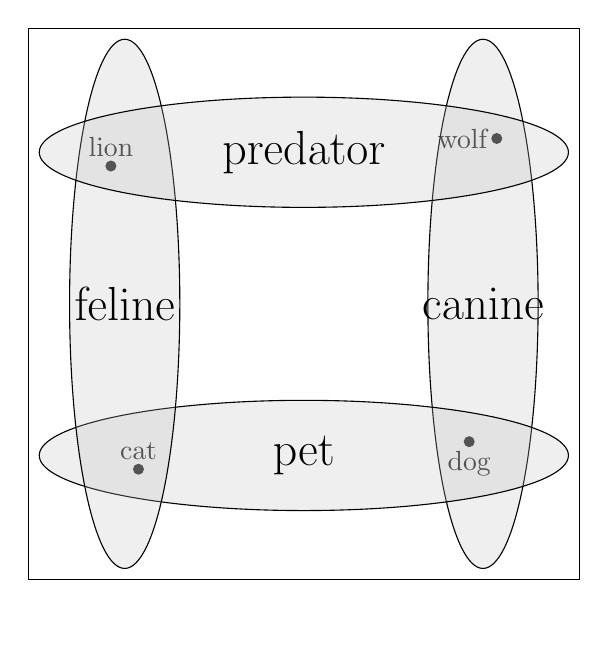
\begin{tikzpicture}[scale=0.07,baseline]
		\draw (0,0)--(-100,0)--(-100,-100)--(0,-100)--(0,0);
    	\draw (-15,-20) [left] node {wolf};
        \fill (-15,-20) circle[radius=1];
        \draw (-20,-75) [below] node {dog};
        \fill (-20,-75) circle[radius=1];
        \draw (-80,-80) [above] node {cat};
        \fill (-80,-80) circle[radius=1];
        \draw (-85,-25) [above] node {lion};
        \fill (-85,-25) circle[radius=1];
        \draw[fill=lightgray, fill opacity=0.25] (-17.5,-50) ellipse (10 and 48);
        \node at (-17.5,-50) {\LARGE canine};
        \draw[fill=lightgray, fill opacity=0.25] (-50,-77.5) ellipse (48 and 10);
        \node at (-50,-77.5) {\LARGE pet};
        \draw[fill=lightgray, fill opacity=0.25] (-82.5,-50) ellipse (10 and 48);
        \node at (-82.5,-50) {\LARGE feline};
        \draw[fill=lightgray, fill opacity=0.25] (-50,-22.5) ellipse (48 and 10);
        \node at (-50,-22.5) {\LARGE predator};
        \node at (-50,-102.5) [single arrow,draw,rotate=90,minimum height=40,minimum width=40,inner sep=15,opacity=0] {};
    \end{tikzpicture}
    \caption{a lexical space}
    \label{fig:bland}
    \end{subfigure}
    \begin{subfigure}[t]{0.5\textwidth}
    \centering
	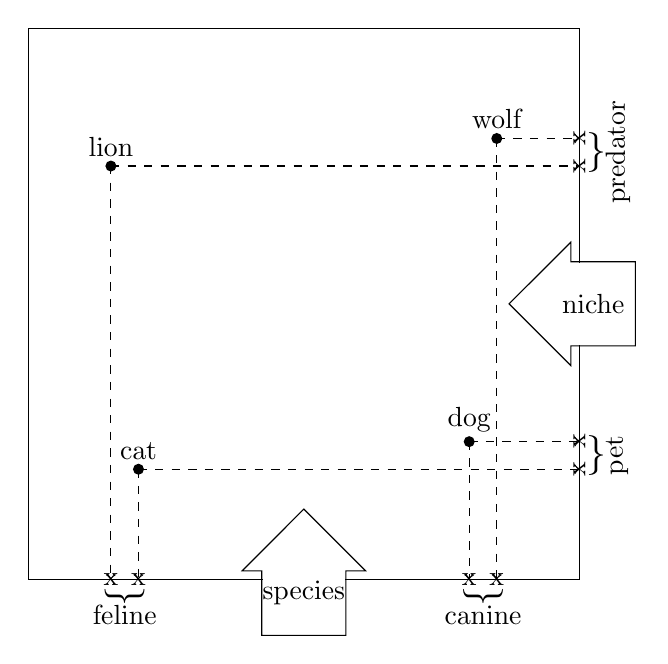
\begin{tikzpicture}[scale=0.07,baseline]
    	\draw (0,0)--(-100,0)--(-100,-100)--(-57.5,-100);
        \draw (-42.5,-100)--(0,-100)--(0,-57.5);
        \draw (0,-42.5)--(0,0);
    	\draw (-15,-20) [above] node {wolf};
        \fill (-15,-20) circle[radius=1];
        \draw[dashed,->] (-15,-20)--(-15,-100);
        \draw (-15,-100) node {x};
        \draw[dashed,->] (-15,-20)--(0,-20);
        \draw (0,-20) node [rotate=90] {x};
        
        \draw (-20,-75) [above] node {dog};
        \fill (-20,-75) circle[radius=1];
        \draw [dashed,->] (-20,-75)--(-20,-100);
        \draw (-20,-100) node {x};
        \draw [dashed,->] (-20,-75)--(0,-75);
        \draw (0,-75) node [rotate=90] {x};
        
        \draw (-80,-80) [above] node {cat};
        \fill (-80,-80) circle[radius=1];
        \draw [dashed,->] (-80,-80)--(-80,-100);
        \draw (-80,-100) node {x};
        \draw [dashed,->] (-80,-80)--(0,-80);
        \draw (0,-80) node [rotate=90] {x};
        
        \draw (-85,-25) [above] node {lion};
        \fill (-85,-25) circle[radius=1];
        \draw [dashed,->] (-85,-25)--(-85,-100);
        \draw (-85,-100) node {x};
        \draw [dashed,->] (-85,-25)--(0,-25);
        \draw (0,-25) node [rotate=90] {x};
        
        \node at (3,-22.5) [below,rotate=90] {predator};
        \node at (3,-22.5) {\Large\}};
		
        \node at (3,-77.5) [below,rotate=90] {pet};
        \node at (3,-77.5) {\Large\}};
		
        \node at (-17.5,-103) [below] {canine};
        \node at (-17.5,-103) [rotate=-90] {\Large\}};

        \node at (-82.5,-103) [below] {feline};
        \node at (-82.5,-103) [rotate=-90] {\Large\}};
        
        \node at (-50,-102.5) [single arrow,draw,rotate=90,minimum height=40,minimum width=40,inner sep=15] {};
        \node at (-50,-102.5) {species};
        \node at (2.5,-50) [single arrow,draw,rotate=180,,minimum height=40,minimum width=40,inner sep=15] {};
        \node at (2.5,-50) {niche};
    \end{tikzpicture}
    \caption{a contextual projection}
    \label{fig:reduce}
    \end{subfigure}
  \caption{In the two-dimensional space depicted in (a), the conceptual vagary of four words maps to overlapping, elongated and indeterminate spaces.  In (b), two different perspectives on the lexical space, represented by the arrows labelled \emph{niche} and \emph{species}, offer contextualised projections in one-dimensional clusters which remit conceptual clarity.}
\label{fig:perspective}
\end{figure}

Furthermore, the high dimensionality of vector space models of distributional semantics in particular should afford precisely these types of contextual viewpoints on potential relationships between words.  Rather than depending on \emph{a priori} disambiguation based on clustering or observations of context in the form of existing combinations of words, I propose that a technique for defining semantic subspaces \emph{in situ} will capture the momentary and situated way in which concepts come about in the course of a cognitive agent's entanglement with the world.  The way that relationships between words coalesce and then dissolve as we change our perspective on the space of this model is designed to reflect the way that concepts emerge dynamically in response to unfolding events in the world, and the ability to selectively specify the dimensional profile of a space of geometrically related semantic representations should enable just this kind of shifting of conceptual perspective.  The theoretical mechanisms for making choices about multi-dimensional perspectives in semantic spaces will be discussed in the next section.

\paragraph{A Note on \emph{Context}} The term \emph{context} has been used widely and varyingly by authors in both theoretical and computational linguistics, and with good reason, as various sense of the concept of context are clearly at play in any serious discussion of the interplay between language and cognition.  Statistically minded computational linguists in particular, of whom I would like to count myself as one, have often used \emph{context} to refer to the window of co-occurrence in which a word token is observed within a sample of text.  In his description of a co-occurrence statistic for measuring semantic similarity, \cite{Schutze1992b} introduced the term \emph{context space} to refer to a space of co-occurrence dimensions, a terminology subsequently adopted by \cite{BurgessEA1997} in relation to their HAL system.  This notion of proximity within a text as context has persevered in the natural language processing literature.

Theoretical linguists and cognitive scientists, on the other hand, have tended to treat \emph{context} as a much more general condition wrapped up with the entire perceptual, phenomenological aspect of existing as a cognitive agent in a complex world.  So for instance \citeauthor{Bateson1972} says that ``message material, or information, comes out of a context into a context,'' \cite[][p. 404]{Bateson1972}, meaning that there is an alignment between the inner context of an agent and the outer context of the world, while \citepos{Grice1975} notion of \emph{implicature} holds that meaning is somehow always determined in a context, with the exact nature of context remaining somewhat open-ended, and this nomenclature has been carried on by subsequent researchers interested in the idea that cognition, conceptualisation, and, correspondingly, language are always in some way specified by a situation in the world.  The idea is that context is probably something that exists in large part outside of language, and almost certainly outside the informationally restrictive confines of word co-occurrences within a sentence.

In this thesis, which seeks to address both those components of language measurable by an information processing system and the more general question of meaning as an environmentally situated phenomenon, I will endeavour to use the term \emph{context} strictly in reference to the latter notion of the situation in which concepts and semantics emerge in tandem.  With regard to words observed in proximity to one another, on the other hand, I will refer to \emph{co-occurrence}, and so additionally to a \emph{co-occurrence window} within which such observations are made and correspondingly a \emph{co-occurrence statistic} as a measure of the relative frequency of such observations.  Hopefully this terminological commit will serve to avoid confusion.

\section{Literal Dimensions of Co-Occurrence}
The model presented here is grounded within the paradigm of distributional semantics, which means that the conceptual geometries that it constructs are the product of observations of word co-occurrences in a large-scale corpus of textual data represented statistically.  Two procedurally distinct methodological regimens have emerged from the recent study of distributional semantics.  The first, and more established, approach involves tabulating word co-occurrence frequencies and then using some function over these to build up word-vector representations.  With roots in the frequentist analysis described by \cite{SaltonEA1975}, recent research has typically involved matrix factorisation techniques presented as either (or both) an optimisation method \citep{BullinariaEA2012} or a noise reducing mechanism \citep{KielaEA2014}.\footnote{\cite{BullinariaEA2012}, \cite{LapesaEA2013}, and \cite{KielaEA2014} have all reported that dimensional reduction techniques including SVD, random indexing, and top frequency feature selection generally do not improve results on word similarity and composition tests, with some notable parameter specific exceptions.}  A more recent approach, which has received a great deal of attention with the increasing availability of large-scale data and the corresponding advent of complex neural network architectures, involves using machine learning techniques to iteratively learn word-vector representations in an online, stepwise traversal of a corpus \citep{BengioEA2003,CollobertEA2008,KalchbrennerEA2014}.  \cite{BaroniEA2014} have described the former as \emph{counting} and the latter as \emph{predicting}, but it must be noted that both methods are very much grounded in observations about the co-occurrence characteristics of vocabulary words across large bodies of text.

Another important similarity between these two approaches is that they each in their own way move towards a representation of relationships between word-vectors which is to some extent optimally informative, and, by the same token, abstract.  In the instance of neural network approaches, this is clearly the case due to the fundamental nature of the technique: the dimensions of this variety of model exist as basically arbitrary handles for gradually adjusting the relative positions of vectors, slightly altering every dimension of each vector each time the corresponding word is observed in the corpus.  And, as far as models based on explicit co-occurrence counts are concerned, the favoured technique tends to involve starting with a large, sparse space of raw co-occurrence statistics (frequencies, or, more typically, an information theoretic type metric) and then factorising this matrix using a linear algebraic technique such as singular value decomposition.  The result, in either case, is a space of vectors which exists just for the sake of placing words in a relationship where distance corresponds to a semantic property, consisting of dimensions which can only be interpreted in terms of the way that they allow the model to relate words, not in terms of their relationship to the underlying data.  In fact, \cite{LevyEA2014b} have argued that recently developed neural network approaches just exactly recapitulate the process of matrix factorisation, and that a careful tuning of hyperparameters will generate commensurable results from either type of model.

A key feature of the methodology proposed in this thesis is that it maintains a base space of highly sparse co-occurrence statistics, which, despite their anchoring in the relatively abstract realm of word positions in a digitised corpus, I will describe as \emph{literal} in the sense that they can be interpreted as corresponding to actual relationships between word tokens in the world.  As mentioned in the previous section, a fundamental objective of this methodology is to afford an abundance of potential perspectives on co-occurrence data.  This objective is accomplished by providing a model with a corresponding proliferation of dimensions from which to make projections by way of context specific selections of subsets of dimensions.  Furthermore, by maintaining the literal connection between the dimensions and the underlying data, the methodology likewise sustains a mechanism for selecting the dimensions in a way that is fundamentally interpretable, in that we can predict something about the geometric contribution of a given dimension to a subspace based on the types of words which tend to co-occur with that dimension.  The co-occurrence profiles of the dimensions themselves will become an important criterion for dimensional selection, and having a very large set of such profiles to analyse will give a semantic model great scope in its capacity for adopting situational perspectives on the relationships between words.

%I don't wish to claim that there is scope for completely or even mainly recapitulating a nuanced conceptual model from the data available in a purely textual environment; to do so would be to move towards claims that intentionality can emerge from rule-based operations on symbols, and the problems with this have been explored by \citepos{Searle1980} Chinese room argument and a subsequent generation of philosophers \citep{PrestonEA2002}.  But I would like to suggest that by building a base model that maintains the accessibility of unreduced co-occurrence information, we likewise maintain the ability to manipulate this base model extemporaneously, in reaction to the ongoing emergence of new contextual information.  The idea is that such a base model would essentially represent the superset of all possible dimensions available for \emph{ad hoc} selection in the course of a 

So the proper framework for describing the model to be examined in this thesis is not so much a single space of word-vectors as a Grassmannian lattice consisting of the power set of all possible combinations of the dimensions characterising the base space.  At the top of this lattice -- the \emph{join} -- sits a single $d$-dimensional space consisting of every available one of the $d$ co-occurrence terms observed throughout the underlying corpus.  At the bottom of the lattice -- the \emph{meet} -- sit $d$ different one-dimensional spaces, each space corresponding to a single co-occurrence term.  If the meet is considered layer-$1$ of the lattice, and the join is considered layer-$d$, then any given interstitial layer-$j$ consists of every possible combination of $j$ dimensions of co-occurrence statistics.  A diagram of a very simple example of one such model is presented in Figure~\ref{fig:lattice}, illustrating the possible subspaces projected from a vastly simplified model consisting of just three co-occurrence dimensions (these particular spaces will be explored in the next section, providing the basis for the interpretable geometries illustrated in Figure~\ref{fig:instruments}).

\begin{figure}
\centering
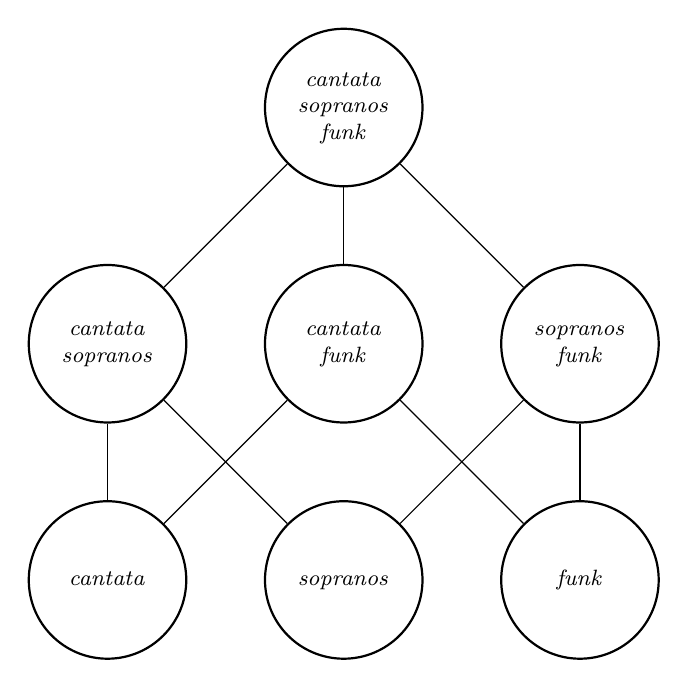
\begin{tikzpicture}[node distance=3cm,every node/.style={draw=black,thick,circle,inner sep=0pt}]
  \footnotesize
  \node[minimum size=2cm](join) {\begin{tabular}{c}
    \emph{cantata} \\
    \emph{sopranos} \\
    \emph{funk}
  \end{tabular}};
  \node[minimum size=2cm](two2) [below of=join] {\begin{tabular}{c}
    \emph{cantata} \\
    \emph{funk}
  \end{tabular}};
  \node[minimum size=2cm](two1) [left of=two2] {\begin{tabular}{c}
    \emph{cantata} \\
    \emph{sopranos}
  \end{tabular}};
    \node[minimum size=2cm](two3) [right of=two2] {\begin{tabular}{c}
    \emph{sopranos} \\
    \emph{funk}
  \end{tabular}};
  \node[minimum size=2cm](one2) [below of=two2] {\begin{tabular}{c}
    \emph{sopranos}
  \end{tabular}};
  \node[minimum size=2cm](one1) [left of=one2] {\begin{tabular}{c}
    \emph{cantata}
  \end{tabular}};
  \node[minimum size=2cm](one3) [right of=one2] {\begin{tabular}{c}
    \emph{funk}
  \end{tabular}};
  \draw (two1)--(join);
  \draw (two2)--(join);
  \draw (two3)--(join);
  \draw (one1)--(two1);
  \draw (one1)--(two2);
  \draw (one2)--(two1);
  \draw (one2)--(two3);
  \draw (one3)--(two2);
  \draw (one3)--(two3);
\end{tikzpicture}
\caption{A lattice of three dimensions, including the two-dimensional subspaces which are used for analysing the conceptual geometry of a small set of word-vectors in Figure~\ref{fig:instruments}}
\label{fig:lattice}
\end{figure}

An important distinction must be drawn, however, between the representation of my model as a lattice and the use of manifolds as an inferential mechanism.  Formal concept analysis in particular has made a productive discipline out of applying lattice type structures to conceptual modelling, using the semi-hierarchical properties of lattices to capture logical relationships of entailment \citep{Wille1982}.  That body of work takes as given that concepts are ``the basic units of thought formed in dynamic processes within social and cultural environments,'' \citep[][p. 2]{Wille2005}.  \cite{Widdows2004} offers a broad overview of how this approach might be pursued through corpus linguistic techniques, while \cite{GeffetEA2005} and, more recently, \cite{KartsaklisEA2016} have proposed statistical techniques using \emph{feature inclusion} metrics to assess the potential entailment relationships between candidate words and corresponding concepts.  The assumption inherent in this interesting work is that words are in some sense supervenient upon the concepts they denote, and that the statistical features of a language will by and large recapitulate the conceptual structure upon which it sits.

As \cite{Rimell2014} has pointed out, however, it is problematic to assume that a spectrum of co-occurrence alone can indicate relationships of hyponymy and hypernymy.  It stands to reason, for instance, that a word with a taxonomically specific denotation such as \emph{bulldog} should probably have a co-occurrence profile including words omitted from the corresponding profile of a word like \emph{lifeform}, which has an ostensibly more general extension---even excluding some of the ambiguity inherent in \emph{bulldog}, it seems reasonable to talk about a \emph{pet bulldog} but less so to talk about a \emph{pet lifeform}, for instance.  Rimell has proposed a measure of change in \emph{topic coherence} as word-vectors are combined algebraically in order to detect entailment relationships.  This measuring is achieved specifically through a process of dimension-by-dimensions comparison between potentially related word-vectors, in particular the \emph{vector negation} method described by \cite{Widdows2003}, combined with topic modelling techniques to analyse the coherence of features distilled by the selectional process.

The methodology proposed in this thesis adheres to the same principle of fine-grained cross-dimensional analysis described by Rimell.  In addition to the practical issues raised by Rimell, my approach is also designed to remain pointedly uncommitted to any claim that concepts are atomic or elementary to thought, or that language and concepts are involved in any kind of strictly hierarchical interrelationship.  Instead, my models operate through an analytical traversal of lattices of subspaces in search of combinations of dimensions that capture conceptually \emph{salient} profiles of co-occurrence features.  If a consequence of this stance is that a model built from this methodology can't be understood in terms of nested, ordered relationships, though, then the question of how conceptual relationships do emerge situationally from the methodology remains.  The next section of this theoretical overview will examine how the actual geometry of a projected subspace itself is expected to do this conceptual work.

\section{Interpretable Geometry}
It is important at this point to distinguish between two different modes of interpretability at play within the operation of the methodology I'm proposing.  On the one hand, we have the process for selecting subspaces described above: this process requires a model composed of tractable dimensions of statistics that can be interpreted based on expectations generated from an analysis of some sort of contextually relevant information.  Some specific mechanisms for this process will be discussed in the next chapter.  Then on the other hand, once this selectional process has taken place, we find ourselves with a subset of dimensions defining a specific subspace.  My claim is that, given the correct selectional criteria for performing this projection -- this traversal of our lattice of vector spaces -- we should be able to generate a subspace in which the projected word-vectors will be interpretable in terms of the actual geometric features of this subspace.

The idea of exploiting the geometry of a transformed space of word statistics is not new.  Indeed, seminal work on latent semantic analysis was motivated by precisely the insight that a singular value decomposition of a high-dimensional, sparse matrix of statistical data about word co-occurrences would result in a dense lower dimensional matrix in which dimensions characterise \emph{latent semantics} rather than literal word co-occurrences \citep{DeerwesterEA1990}.  Thus the linear algebraic methodology of generating a lower dimensional matrix of optimally informative dimensions arguably transforms a space of specific co-occurrence tendencies into a space of more general conceptual relationships.  In fact, \citeauthor{LandauerEA1997} have subsequently argued that the dimensional reduction by way of factorisation itself might directly mirror cognitive conditioning, modelling the way that the mind can ``correctly infer indirect similarity relations only implicit in the temporal correlations of experience,'' \citep[][p. 212]{LandauerEA1997}.

Of course the dimensions of a factorised matrix are still not interpretable in themselves.  They are, rather, an optimal abstraction of the underlying data, in which each dimension is maximally informative -- and, accordingly, orthogonal -- in comparison to the other dimensions.  What we desire in a model, however, is a mechanism for actually interpreting directions and regions within a subspace projected by the model.  This objective is motivated by \citepos{Gardenfors2000} insight into the inferential power of \emph{conceptual spaces}: by building spaces in which the dimensions themselves correspond to \emph{properties}, G\"{a}rdenfors has illustrated how features of points and regions within these spaces such as convexity and betweeness can be interpreted as corresponding to conceptual membership and can accordingly be used to reason about relationships between concepts.  In more recent work, motivated by psycholinguistic insight into the significance of the \emph{intersubjectivity} by which language facilitates the mutual ascription of cognitive content between interlocutors, \cite{Gardenfors2014} has proposed that semantics are derived from a communicative alignment of conceptual spaces.

A classic example of a G\"{a}rdenforsian conceptual space is the space of colours, which can be defined in terms of, for instance, hue, brightness, lightness, and colourfulness: any colour percept can be specified as a point corresponding to coordinates along each of these dimensions.  Moreover, regions within the space of colours can be defined geometrically: the concept \textsc{red} will correspond to a convex region within the space, and any point lying between two points known to be labelled \emph{red} will likewise be considered \textsc{red}.  \cite{Jager2010} has devised an experiment mapping linguistic descriptions to conceptual regions precisely within the domain of colours.  Taking a large set of multi-lingual data regarding colour naming conventions and treating each of 330 different colours as an initially independent dimension, J\"{a}ger demonstrated how an extrapolation of optimally informational dimensions via a principle component analysis revealed clusterings of colour names into convex regions.\footnote{The cross-cultural universality of colour naming conventions presented by \cite{KayEA1999}, which J\"{a}ger takes as a basis for his research, is controversial to say the least -- see \cite{Levinson2001} for an alternative point of view -- but J\"{a}ger's work remains a good example of a computational technique for extrapolating conceptual spaces from quantitative linguistic data.}

Similarly motivated by G\"{a}rdenfors's model of conceptual spaces, \cite{DerracEA2015} have built vectors of domain specific documents, associating word frequencies within documents with document labels.  A multi-dimensional scaling procedure is then used to project these document-vectors into a Euclidean space in which the authors predict that properties such as \emph{parallelness} and \emph{betweeness} will correspond to conceptual relationships between documents.  The authors demonstrate that geometry in their projected spaces does indeed afford conceptual interpretation: the vector they construct from large scale textual data for the word \emph{bog} is found to be more or less between the vectors for \emph{heath} and \emph{wetland}, for instance, and the vector for the film \emph{Jurassic Park} lies in directions associated with \textsc{dinosaurs} and \textsc{special effects}.  This work is particularly notable in that \citeauthor{DerracEA2015} appreciate the significance of projecting spaces which are interpretable in terms of Euclidean distances rather than simply the cosine similarity of vectors extending from the origin of a space: Euclidean metrics provide a platform for more nuanced considerations of the relationships between points.

The type of space exemplified by the research of J\"{a}ger and \citeauthor{DerracEA2015} is moving towards being a conceptual space in the way that its geometry offers itself up to semantic interpretation, but importantly these remain static spaces comprised of abstract dimensions, albeit dimensions generated in order to optimise the interpretability of the spaces they delineate.  The objective of my model is to emulate the geometric interpretability of these other spaces in an extemporaneous, contextually dynamic way.  To illustrate this point, consider the two spaces illustrated in Figure~\ref{fig:instruments} (taken from real co-occurrence data, as described in the next chapter, and based on the lattice of subspaces illustrated in Figure~\ref{fig:lattice}).  Here co-occurrence statistics are used to define three different dimensions, from which two different two-dimensional subspaces are selected with word-vectors plotted into each subspace.  In each subspace, a particular conceptual geometry emerges, oblique to the axes of each subspace but nonetheless indicating distinct conceptual regions in which words align themselves in an interpretable way.

\begin{figure}[t]
	\begin{subfigure}[t]{0.5\textwidth}
    \centering
	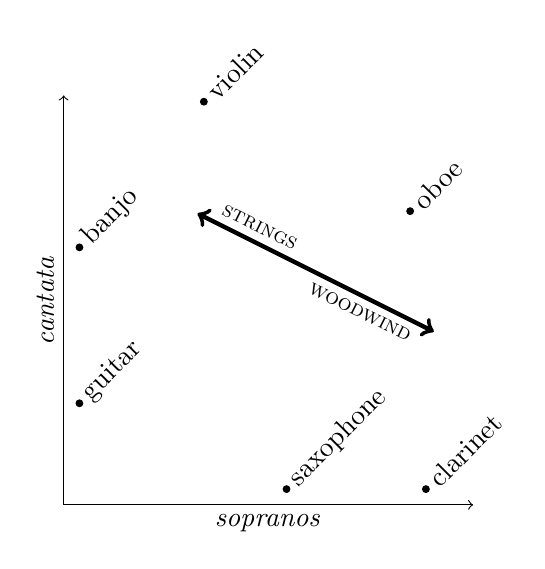
\begin{tikzpicture}[scale=1,baseline]
		\draw [->] (-0.2,-0.2)--(5,-0.2);
		\draw [->] (-0.2,-0.2)--(-0.2,5);
		\node at (2.4,-0.2) [below] {\emph{sopranos}};
		\node at (-0.2,2.4) [above,rotate=90] {\emph{cantata}};
		\draw [<->,ultra thick] (1.5,3.5)--(4.5,2);
		\node at (2.2,3.15) [above,rotate=-26.57] {\footnotesize \textsc{strings}};
		\node at (3.65,2.425) [below,rotate=-26.57] {\footnotesize \textsc{woodwind}};
		\node at (0.0,1.09) [right,rotate=45] {guitar};
		\fill (0.0,1.09) circle[radius=0.05];
		\node at (0.0,3.07) [right,rotate=45] {banjo};
		\fill (0.0,3.07) circle[radius=0.05];
		\node at (1.58,4.92) [right,rotate=45] {violin};
		\fill (1.58,4.92) circle[radius=0.05];
		\node at (2.63,0.0) [right,rotate=45] {saxophone};
		\fill (2.63,0.0) circle[radius=0.05];
		\node at (4.40,0.0) [right,rotate=45] {clarinet};
		\fill (4.40,0.0) circle[radius=0.05];
		\node at (4.20,3.53) [right,rotate=45] {oboe};
		\fill (4.20,3.53) circle[radius=0.05];
    \end{tikzpicture}
    \caption{\textsc{strings} vs \textsc{woodwind}}
    \label{fig:svsw}
    \end{subfigure}
    \begin{subfigure}[t]{0.5\textwidth}
    \centering
	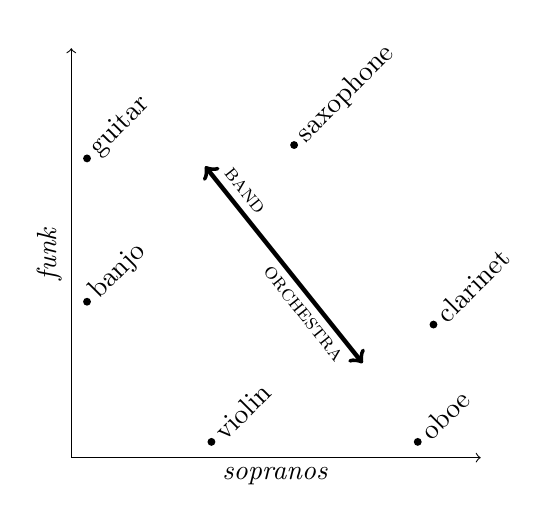
\begin{tikzpicture}[scale=1,baseline]
		\draw [->] (-0.2,-0.2)--(5,-0.2);
		\draw [->] (-0.2,-0.2)--(-0.2,5);
		\node at (2.4,-0.2) [below] {\emph{sopranos}};
		\node at (-0.2,2.4) [above,rotate=90] {\emph{funk}};
		\draw [<->,ultra thick] (1.5,3.5)--(3.5,1);
		\node at (1.85,3.0625) [above,rotate=-51.35] {\footnotesize \textsc{band}};
		\node at (2.9,1.75) [below,rotate=-51.35] {\footnotesize \textsc{orchestra}};
		\node at (0.0,3.60) [right,rotate=45] {guitar};
		\fill (0.0,3.60) circle[radius=0.05];
		\node at (0.0,1.78) [right,rotate=45] {banjo};
		\fill (0.0,1.78) circle[radius=0.05];
		\node at (1.58,0.0) [right,rotate=45] {violin};
		\fill (1.58,0.0) circle[radius=0.05];
		\node at (2.63,3.77) [right,rotate=45] {saxophone};
		\fill (2.63,3.77) circle[radius=0.05];
		\node at (4.40,1.49) [right,rotate=45] {clarinet};
		\fill (4.40,1.49) circle[radius=0.05];
		\node at (4.20,0.0) [right,rotate=45] {oboe};
		\fill (4.20,0.0) circle[radius=0.05];
    \end{tikzpicture}
    \caption{\textsc{band} vs \textsc{orchestra}}
    \label{fig:bvso}
    \end{subfigure}
  \caption{Based on real co-occurrence data, swapping one dimension in a two-dimensional subspace reveals two different conceptual geometries.}
  \label{fig:instruments}
\end{figure}

The first thing to note about these spaces is the way that swapping a single dimension in a two dimensional subspace can have a significant impact on the conceptual affordances of the subspace's geometry.  Realigning the relationships between terms along a single axis leads to a complete shift in the groupings of terms, and, correspondingly, to the interpretation of regions and directions.  If these are conceptually sound subspaces, then we might expect word-vectors found within the area of the triangle described by the points labelled \emph{guitar}, \emph{banjo}, and \emph{violin} in Figure~\ref{fig:svsw} to be the names of other string instruments, or other conceptually relevant terms.  This is possibly asking too much of a subspace consisting of data regarding co-occurrences with just two terms across a large scale corpus, but as we scale up the dimensionality of the space -- as we ascend the lattice of subspaces of a fully realised model -- we can expect proper conceptual spaces to begin to coalesce.

The next thing to note is that the dimensions themselves are not especially interpretable.  While these dimensional profiles are explicable -- and indeed the ability to trace these statistics back to the corpus might turn out to be a desirable property for some applications -- the dimensions themselves do not conform to \citepos{Gardenfors2000} notion of dimensions as representing the properties that compose a concept.  It might be surprising, for instance, that the word \emph{cantata} has a higher propensity for co-occurrence with the word \emph{banjo} than with the word \emph{clarinet}, given that cantatas have traditionally included parts for the latter but not the former.  An examination of the underlying data, extracted, as described in the next chapter, from English language Wikipedia, reveals that the term \emph{cantata} has been adopted, perhaps somewhat figuratively, by some bluegrass musicians, and so co-occurrences with \emph{banjo} are indeed observed.

Rather than consider such usage as anomalous or attempt some sort of \emph{a priori} word sense disambiguation, I propose to embrace the haphazardness of language and use it as a tool for projecting conceptually productive geometries.  In fact it would be surprising if it turned out that in anything other than the most specialised cases we could simply pick dimensions based on their labels and then expect co-occurrence statistics to play out in a conceptually coherent way, as this would contradict the Relevance Theoretic thesis that language in use is always significantly underspecified.  With this in mind, I suggest that we consider some set of dimensions, delineating a subspace and the corresponding geometry of word-vectors, to map precisely to a given context, and to effectively serve as the connective structure between language and conceptualisation.  Under this regimen, the dimensions themselves become the constitutive substance of a context, but they do not compositionally define any context in which they participate; rather, the contextualisation is an emergent property of the combination of dimensions underwriting it, corresponding to \emph{a way of speaking} about things.

The spaces illustrated in Figure~\ref{fig:instruments} are the product of a survey of a lattice consisting of combinations of just three dimensions, and as such the conceptual affordances of this toy model are highly limited.  As we add dimensionality to the model, however -- as we observe more terms co-occurring with our vocabulary of word-vectors -- we can expect an exponential growth in the combinatory possibilities of subspace construction.  With enough dimensions from which to choose, and with an appreciable degree of variance between the profiles of each dimensions, there should be scope for projecting more or less any constellation of word-vectors we desire.  The next question, then, is how to go about actually extracting a high dimensional base model of co-occurrence statistics from a large scale textual corpus and then explore the conceptual possibilities of this base space's inherent subspaces.  The next chapter will answer this question.

%\section{A Computational Process}
%In this final section of this chapter, a technical implementation of the model described throughout the preceding three sections will be explained in detail.

%\subsection{A Large Scale Textual Corpus}
%The first step in a corpus based approach to natural language processing is the selection of the data which will provide the basis for our model.  I've picked the English language portion of Wikipedia as my data source, a choice which is in accordance with a good deal of work done in the field.  Some authors 

%In the case of the model used throughout this thesis, the November 2014 dump of English language Wikipedia has been used.\footnote{Accessible at XXX}  A data cleaning process has been implemented, the first step of which is the chunking of the corpus into individual sentences.  Next parenthetical phrases are removed from each sentence, as these can potentially skew co-occurrence data, and all other punctuation is subsequently removed.  All characters are converted into lowercase to avoid words capitalised at the beginning of sentences, quotations, and other places from being considered as unique types.  Finally, the articles \emph{a}, \emph{an}, and \emph{the} are removed as they can distort co-occurrence windows (consider, for instance, how these terms affect the proximity of the other words in the phrase ``a mouse, an owl, and a dog sat on the moon'').  The cleaned corpus contains about

%-WORD, SENTENCE COUNTS

%As is generally the case with data cleaning, these measures are prone to error: for instance, due to the removal of punctuation, the contraction \emph{we're} will be considered identical to the word \emph{were}.  One of the strengths of the subspace projection technique that my model uses is its resilience to noise.  So, for instance, misspellings will be categorised as highly anomalous co-occurrence dimensions and are therefore unlikely to be contextually selected -- or, if they are regularly encountered enough to be contextually significant, there may well be useful information in the co-occurrence profile of such mistakes -- and essentially ubiquitous words are unlikely to provide context specific information, so the ambiguity between \emph{we're} and \emph{were} is unlikely to be drawn into any of the subspaces actually projected by the model.

%From the cleaned corpus, the model's vocabulary is defined as the top 200,000 most frequently occurring word types.  This cut-off point is very close to the point where the total number of word tokens included -- that is, occurrences of any word of any type -- included by selecting all instances of all vocabulary words equals the total number of word types -- that is, unique word forms -- excluded.  Given the Zipfian distribution of word frequencies as observed throughout the corpus, this means that more than 95\% of the co-occurrence data available from the corpus will be taken into account by the model, while the number of word-vectors used to express this data represents less than 5\% of the potential vocabulary---a fairly efficient way of extrapolating statistics from the corpus.

%- human vocabulary size

%\subsection{Mutual Information of Word Co-Occurrences}
%The critical event in the 

%Here, following the example of almost all distributional semantic work, co-occurrence between a word $w$ and another word $c$ will be considered in terms of the number of other words between $w$ and $c$.  In the case of my model, again in accord with the a great deal of work within the field, a statistic for word $w$ in terms of its co-occurrence with $c$ will be derived from the consideration of all the times that $c$ is observed within $k$ words of $w$, where $k$ is one of the primary model parameters that will be considered in the experiments reported in later chapters of this thesis.  Based on these co-occurrence events, a matrix $M$ is defined, where rows consist of word-vectors, one for each of the 200,000 words in the vocabulary, and columns correspond to terms with which these vocabulary words co-occur.  These column-wise co-occurrence dimensions include the words in the vocabulary, including the possible co-occurrence of a word with itself (``a \emph{rose} is a \emph{rose} is a \emph{rose}'', for instance) as well as many, many words that are not in the vocabulary, to the extent that every word type in the corpus is considered as a dimension of co-occurrence.

%In this last respect, my model diverges from the typical approach, which usually seeks to limit not only the vocabulary but also the dimensionality of the underlying co-occurrence matrix.  This has typically involved a curtailing of the number of co-occurrence terms at both ends of the frequency spectrum, based on the assumption that both high frequency so-called function words (the prepositions, conjunctions, and so forth) and low frequency terms such as obscure proper names will muddy a model with either general flattening or highly topical skewing.  In the case of my model, however, these problems are irrelevant, as dimensions will be selected on a case-by-case, context specific basis, and there is no good reason to discard information which may in some possibly unforeseen circumstance prove relevant.  The result is a 200,00 by $\approx$ 7.5 million matrix $M$ where a scalar corresponding to co-occurrences between $w$ and $c$ is defined in terms of this equation:

%\begin{equation}\label{eq:MI}
%M_{w,c} = \log_2 \left(\frac{n_{w,c} \times W}{n_w \times \left(n_c + a\right)} + 1\right)
%\end{equation}

%Here $n_{w,c}$ represents the total number of times that that $c$ is observed as co-occurring in a sentence within $k$ words on either side of $w$, $n_w$ is the independent frequency of occurrences of $w$, and $c$ is likewise the overall frequency of $c$ being observed as a co-occurrence term throughout the corpus.  $W$ is the overall occurrence of all words throughout the corpus---and it should be noted that, excluding the term $a$, the ratio in Equation~\ref{eq:MI} is equivalent to the joint probability of $w$ and $c$ co-occurring.  The application of a logarithm to this ratio, again a common practice, is in the spirit of \citepos{Shannon} information theory, and is 

%The term $a$ is a skewing constant used to prevent highly specific co-occurrences from dominating the analysis of a word's profile, set for the purposes of the work reported here at 10,000.\footnote{Anecdotally, the first combination of input words analysed during an early stage of the development of this model that didn't use a smoothing constant was the phrase ``musical creativity'', and the very first dimension indicated by the analysis was labelled \emph{gwiggins}---my primary supervisor's email handle.  Prof. Wiggins's deep connection with music and creativity meant that every instance of \emph{gwiggins} occurring throughout Wikipedia was in the vicinity of both \emph{musical} and \emph{creativity}, and so the dimension was indicated by the combination of these terms, which makes sense, but it was still a bit eerie to have such a personally relevant result generated by a model based on such general data.}

%Finally, the entire ratio is skewed by 1 so that all values returned by the logarithm will be greater than 0, with a value of zero therefore indicating that two words have never been observed to co-occur with one another.  This is again a departure from standard practice, where, in word counting models, a \emph{pointwise mutual information} mechanism involving not skewing the ratio and instead treating any ratio of frequencies less than 1 -- that is, any co-occurrence that is observed less than often than balance of the mean values for all occurrences of $w$ and all co-occurrences with $c$ -- as being equivalent to 0, or no co-occurrence at all.  The motivation for this more typical technique is again to avoid incorporating unnecessary and potentially confounding information into a model, but, again, in the case of my model, the dimensional selection process will tend to ignore such information, and at the same time, as will be seen, data regarding relatively unlikely co-occurrences can sometimes also be quite informative.  In support of my technique, it is worth mentioning that the vast majority of potential co-occurrences will never be observed, and, at the same time, a comprehensive language model should maintain at least the possibility of any co-occurrence

%\cite{Brown}

%so there seems to be wisdom in the idea of not throwing away information about even relatively unlikely linguistic events.

%\subsection{Dimensional Selection Techniques}
%Having established a base model of co-occurrence statistics, the 

%\begin{equation}\label{eq:oldNorm}
%w^j_i = \frac{w^j_i}{\sqrt{\sum_{k=1}^{b} \left(w^k_i\right)^2}}
%\end{equation}

%\begin{equation}\label{eq:Norm}
%w^j_i = \frac{w^j_i}{\sum_{k=1}^{b} abs\left(w^k_i\right)}
%\end{equation}

%\begin{equation}\label{eq:Arg}
%\mu_c =  \frac{1}{n} \sum_{w=1}^{n}N_{w,c}
%\end{equation}

%\begin{equation}\label{eq:Trans}
%M_{w,c} \Rightarrow S_{w,c'}
%\end{equation}
%\subsection{Extracting Semantics from Geometric Features}

%\chapter{A Computational Implementation of Context Sensitive Distributional Semantics} \label{chap:method}
In the previous chapter, I laid the theoretical groundwork for a distributional semantic methodology for dynamically establishing perspectives on statistical data about language use.  In this chapter, I'll describe the technical details for building a computational implementation of such a methodology.  The objective of this implementation is to establish a rigorous procedure for generating subspaces of word vectors, based on observations of word co-occurrences in an underlying corpus, the geometries of which are semantically productive in particular contexts.  This will involve three steps:

\begin{enumerate}
\item The selection, processing, and analysis of a large scale textual corpus in order to create a high dimensional base space of co-occurrence statistics;
\item The development of techniques for selecting lower dimensional subspaces based on some sort of contextualising input;
\item The exploration of the geometry of the projected subspaces in search of semantic correlates.
\end{enumerate}

The following three sections will pursue each of these aspects of a technical implementation in turn.  The end result is effectively a mapping from text as raw data to geometry as semiotic generator.  A fourth section will describe an alternative, general interpretation of the statistical data which underwrites my models and additionally offer a brief overview of another distributional semantic methodology, all to be used as a point of comparison in the empirical results which will be discussed in subsequent chapters.

\section{Establishing and Analysing a Large Scale Textual Corpus}
The first step in a corpus based approach to natural language processing is the selection of the data which will provide the basis for our model.  I've picked the English language portion of Wikipedia as my data source, a choice which is in accordance with a good deal of work done in the field.  For instance, \cite{GabrilovichEA2007} and \cite{CollobertEA2008}, to name just a couple, use Wikipedia as their base data for training distributional semantic models designed to perform tasks similar to the ones explored in subsequent chapters, while \cite{Baroni2014}, \cite{PenningtonEA2014}, and \cite{GutierrezEA2016} use amalgamated corpora that include Wikipedia as a major component.  Wikipedia provides a very large sample of highly regular language, meaning that we can expect a certain syntactic and semantic consistency as well as language which, if not always overtly literal, is likewise not typically abstruse or periphrasitc.  This should supply a source of linguistic data in which, to revisit the central dogma of the distributional hypothesis, words which occur in a specific syntactic and lexical setting can be expected to be semantically similar.

In the case of my implementations, the November 2014 dump of English language Wikipedia has been used.\footnote{Relatively recent Wikipedia dumps are available at \url{https://dumps.wikimedia.org/}.}  A data cleaning process has been implemented, the first step of which is the chunking of the corpus into individual sentences.  Next parenthetical phrases are removed from each sentence, as these can potentially skew co-occurrence data, and all other punctuation is subsequently removed.  All characters are converted into lowercase to avoid words capitalised at the beginning of sentences, quotations, and other places being considered as unique types.  Finally, the articles \emph{a}, \emph{an}, and \emph{the} are removed as they can distort co-occurrence distance counts.  The cleaned corpus contains nearly 1.1 billion word tokens, consisting of almost 7.5 million unique word types.  The distribution of these types is predictably Zipfian: over 10 million occurrences of the top nine word types are observed, while the least frequent 4.27 million words -- more than half of all types -- only occur once.  The top end of this distribution is populated by conjunctions, prepositions, and pronouns, while the bottom end is characterised by obscure place names, one-off abbreviations, unicode representing non-Latin alphabet spellings, and a good many spelling errors.

As is generally the case with data cleaning, these measures are prone to error: for instance, due to the removal of punctuation, the contraction \emph{we're} will be considered identical to the word \emph{were}.  One of the strengths of the subspace projection technique that my methodology uses is its resilience to noise.  So, for instance, misspellings will be categorised as highly anomalous co-occurrence dimensions and are therefore unlikely to be contextually selected -- or, if they are regularly encountered enough to be contextually significant, there may well be useful information in the co-occurrence profile of such mistakes -- and, at the other end of the spectrum, essentially ubiquitous words are unlikely to provide context specific information, so the ambiguity between \emph{we're} and \emph{were} is unlikely to be drawn into any of the subspaces actually projected by the model.

From the cleaned corpus, a model's vocabulary is defined as the top 200,000 most frequently occurring word types.  This cut-off point is very close to the point where the total number of word tokens included -- that is, occurrences of any word of any type -- by selecting all instances of all vocabulary words equals the total number of word types -- that is, unique word forms -- excluded.  Given the Zipfian distribution of word frequencies as observed throughout the corpus, this means that more than 95\% of the co-occurrence data available from the corpus will be taken into account by the model, while the number of word-vectors used to express this data represents less than 5\% of the potential vocabulary---a fairly efficient way of extrapolating statistics from the corpus.  The selection of this as a cut-off point means that the least frequent words in the vocabulary occur 83 times throughout the corpus.

Having processed the corpus and established the target vocabulary, the next step of this methodology is to build up a based space of co-occurrence statistics.  Here, following the example of the majority distributional semantic work, co-occurrence between a word $w$ and another word $c$ will be considered in terms of the number of other words between $w$ and $c$.  In the case of my methodology, and again in accord with the a great deal of work within the field, a statistic for word $w$ in terms of its co-occurrence with $c$ will be derived from the consideration of all the times that $c$ is observed within $k$ words of $w$, where $k$ is one of the primary model parameters that will be considered in the experiments reported in later chapters of this thesis.  Based on these co-occurrence events, a matrix $M$ is defined, where rows consist of word-vectors, one for each of the 200,000 words in the vocabulary, and columns correspond to terms with which these vocabulary words co-occur.  These column-wise co-occurrence dimensions include the words in the vocabulary as well as many, many words that are not in the vocabulary, to the extent that every word type in the corpus is considered as a candidate for co-occurrence.  A \emph{pointwise mutual information} metric gauging the unexpectedness associated with the co-occurrence of two words is calculated in terms of this equation:

\begin{equation}\label{eq:MI}
M_{w,c} = \log_2 \left(\frac{f_{w,c} \times W}{f_w \times \left(f_c + a\right)} + 1\right)
\end{equation}

Here $f_{w,c}$ represents the total number of times that $c$ is observed as co-occurring in a sentence within $k$ words on either side of $w$, $f_w$ is the independent frequency of occurrences of $w$, and $f_c$ is likewise the overall frequency of $c$ being observed as a co-occurrence term throughout the corpus.  $W$ is the overall occurrence of all words throughout the corpus--and it should be noted that, excluding the term $a$, the ratio in Equation~\ref{eq:MI} is equivalent to the joint probability of $w$ and $c$ co-occurring.  The term $a$ is a skewing constant used to prevent highly specific co-occurrences from dominating the analysis of a word's profile, set for the purposes of the work reported here at 10,000.\footnote{Anecdotally, the first combination of input words analysed during an early stage of the development of this model that didn't use a smoothing constant was the phrase ``musical creativity'', and the very first dimension indicated by the analysis was labelled \emph{gwiggins}---the email handle of one of my supervisors.  Prof. Wiggins's deep connection with music and creativity meant that every instance of \emph{gwiggins} occurring throughout Wikipedia was in the vicinity of both \emph{musical} and \emph{creativity}, and so the dimension was indicated by the combination of these terms, which makes sense, but it was still a bit eerie to have such a personally relevant result generated by a model based on such general data.}  Finally, the entire ratio is skewed by 1 so that all values returned by the logarithm will be greater than 0, with a value of zero therefore indicating that two words have never been observed to co-occur with one another.

This last step of incrementing the ratio of frequencies in order to avoid values tending towards negative infinity in the case of very unlikely co-occurrences is again a departure from standard practice, where, in word counting models, a \emph{positive pointwise mutual information} mechanism involving not skewing the ratio and instead treating any ratio of frequencies less than 1 -- that is, any co-occurrence that is observed less often than the balance of the mean values for all occurrences of $w$ and all co-occurrences with $c$ -- as being equivalent to zero, or no co-occurrence at all \citep[][have considered a more general variable ratio shifting parameter]{LevyEA2014b}.  The motivation for this more typical technique is again to avoid incorporating unnecessary and potentially confounding information into a model, but, again, in the case of my model, the dimensional selection process will tend to ignore such information, and at the same time, as will be seen, data regarding relatively unlikely co-occurrences can sometimes also be quite informative.  Other areas for variation in deriving co-occurrence statistics include the nature of the co-occurrence window itself, where some researchers have taken weighted samples \citep or considered word order, and also the actual representation of tokens within the corpus, where part-of-speech and dependency tagging \citep{PadoEA2007} have been applied to positive effect.  \cite{LapesaEA2014} and \cite{MilajevsEA2016} offer comparative overviews of the effects of parameter variations on the performance of distributional semantic techniques.

The net result of my methodology is a matrix of weighted co-occurrence statistics, where higher values indicate a high number of observations of word $w$ co-occurring with word $c$ relative to the overall independent frequencies of $w$ and $c$.  Values of zero indicate words which have never been observed to co-occur in the corpus, and, as most words never co-occur with one another, the matrix is highly sparse.  The weighting scheme results in a kind of semi-normalisation of the matrix: infrequent words will tend to correspond to more sparse dimensions, but the non-zero values along these dimensions will by the same token tend to be higher due to the lower value of the word's frequency in the denominator.  So far this technique sits comfortably within the scope of existing work in the field.  It is what I propose to do with this base matrix that will begin to distinguish my methodology, and this next step in the process of projecting context sensitive spaces of word-vectors will be discussed in the following section.

\section{Selecting Dimensions from a Sparse Co-Occurrence Matrix}
Context has thus far remained a somewhat abstract concept in this thesis.  In principle, the context in which conceptualisation occurs for a cognitive agent is its environment with all its affordances, linguistic and semantic but also more generally perceptual: in a word, the agent's \emph{umwelt} \citep{VonUexkull1957}.  In the world of physical entanglements, language presents itself with precisely the same open-ended opportunities for action as other modes of cognition---and, in the case of language, the action afforded is meaning making.  In practice, however, for the purposes of my methodology, context will be defined lexically, as a word or set of words which are fed to a model, analysed in terms of their co-occurrence profiles, and then used to generate a subspace of conceptually relevant co-occurrence dimensions.  The intuition behind this approach is the idea that there should be a set of words which collectively selects a set of dimensions that are conceptually relevant to some conceptual context, and the geometry of the word-vectors of my model vocabulary as projected into the subspace delineated by this set of dimensions should reveal the semantics of this context.

So, with regard to the present technical description, I will treat \emph{context} as meaning some set of words $T$ which have been selected for the purpose of performing some type of semantic evaluation and act as input to a context sensitive distributional semantic model.  The exact mechanisms for specifying $T$ will be discussed in subsequent chapters with regard to each of the individual experiments to be performed using my methodology; for now, I offer a general outline.  Each component of $T$ points to a word-vector in the matrix $M$ described in the previous section, and the collection of word-vectors corresponding to $T$ serve as the basis for an analysis leading to the projection of a context specific subspace $S$.  I propose three basic techniques for generating these projections, with the model parameter $d$ indicating the specified dimensionality of the subspace to be selected:

\begin{description}
\item[Joint] A subspace of $d$ dimensions with non-zero values for all elements of $T$ and the highest mean PMI values across all elements of $T$ is selected;
\item[Indy] The top $d/|T|$, where $|T|$ is the cardinality of $T$, dimensions are selected for each element of $T$ regardless of their values for other elements of $T$, and then these dimensions are combined to form a subspace with dimensionality $d$;
\item[Zipped] The top dimensions for each element of $T$ are selected as in the \textsc{indy} technique, with the caveat that all selected dimensions must have non-zero values for all elements of $T$ and no dimension is selected more than once.
\end{description}

These techniques are used for the purpose of analysis, and, once this analysis has been performed, the subset of dimensions returned is used to project the entire model vocabulary onto a $d$ dimensional subspace.  The \textsc{joint} technique requires the greatest finesse, as there is an element of cross-dimensional comparison at play.  As such, for the purposes of this technique, the word-vectors selected by $T$ are merged, dimensions with non-zero values for any of the word-vectors are discarded, and the resulting truncated word-vectors, each consisting of an equal number of non-zero dimensions, are normalised.  This ensures that certain elements of $T$ won't dominate the analysis: because the frequency of each word in $T$ applies a deflationary pressure on the PMI values associated with the corresponding word-vectors, very infrequent words would be liable to dominate the analysis with the associated high PMI values in their profile.  This effect is illustrated in Table~\ref{tab:norms}, where PMI values for the words \emph{guitar}, which at 88,285 occurrences is ranked 1541 in frequency, are compared with those for the word \emph{dulcimer}, which occurs 516 times and is ranked 62,313.  Among the dimensions with non-zero values for both words, normalisation brings the respective co-occurrence profiles more in line with one another, facilitating the selection of a subspace which is jointly characteristic of the input terms.

\begin{table}
\centering
\begin{tabular}{llrrlrrlrr}
\hline
& \multicolumn{3}{c}{\emph{guitar}} & \multicolumn{3}{c}{\emph{dulcimer}} \\
& dimension & PMI & normalised & dimension & PMI & normalised \\
\hline
\parbox[t]{2mm}{\multirow{5}{*}{\rotatebox[origin=c]{90}{\textsc{high}}}} & \emph{mandolin} & 8.30964 & 0.10719 & \multicolumn{1}{|l}{\emph{hammered}} & 13.97749 & 0.09354 \\
& \emph{bass} & 8.08501 & 0.10429 & \multicolumn{1}{|l}{\emph{dulcimer}} & 12.73992 & 0.08526 \\
& \emph{12-string} & 8.07679 & 0.10418 & \multicolumn{1}{|l}{\emph{autoharp}} & 11.50399 & 0.07699 \\
& \emph{acoustic} & 7.99076 & 0.10308 & \multicolumn{1}{|l}{\emph{appalachian}} & 11.23224 & 0.07517 \\
& \emph{banjo} & 7.96400 & 0.10057 & \multicolumn{1}{|l}{\emph{zither}} & 10.98302 & 0.07350 \\
\hline
\parbox[t]{2mm}{\multirow{5}{*}{\rotatebox[origin=c]{90}{\textsc{low}}}} & \emph{\emph{attacked}} & 0.05222 & 0.00067 & \multicolumn{1}{|l}{\emph{him}} & 0.25698 & 0.00172 \\
& \emph{report} & 0.04768 & 0.00062 & \multicolumn{1}{|l}{\emph{school}} & 0.25340 & 0.00170 \\
& \emph{country} & 0.04418 & 0.00057 & \multicolumn{1}{|l}{\emph{would}} & 0.23825 & 0.00159 \\
& \emph{champions} & 0.02644 & 0.00034 & \multicolumn{1}{|l}{\emph{into}} & 0.21336 & 0.00143 \\
& \emph{regions} & 0.02538 & 0.00033 & \multicolumn{1}{|l}{\emph{there}} & 0.21320 & 0.00143 \\
\hline
\end{tabular}
\caption{The top five and bottom five dimensions by PMI value for the words \emph{guitar} and \emph{dulcimer}, out of all the dimensions with non-zero values for both words, with scores tabulated independently for each word.}
\label{tab:norms}
\end{table}

In the cases of the \textsc{indy} and \textsc{zipped} techniques, the selectional process is more straightforward, since mean values between word-vectors are not being considered.  Where the \textsc{joint} technique is intended to discover subspaces that represent an amalgamation of the input terms, the \textsc{indy} technique is expected to produce a subspace where individual conceptual characteristics of the input terms, captured as collections of co-occurrence dimensions, are distilled into distinct geometric regions.  The \textsc{zipped} technique might be seen as something of a hybrid of the \textsc{joint} and \textsc{indy} techniques, since it used the \textsc{indy} approach to make selections from the intermediary space of non-zero dimensions available to the \textsc{joint} technique.  In each instance, these techniques are formulated to return a set of dimensions which, with varying degrees of cohesion, delineate a space that is in some sense salient to the contextual terms $T$ serving as the basis for the analysis.  In all cases, these techniques are used for the purpose of analysis, and, once this analysis has been performed, the subset of dimensions returned is used to project the entire model vocabulary onto a $d$ dimensional subspace.

In order to offer a sense of what's happening with these dimensions selection techniques, a preliminary and intuitively motivated case study of dimension selection is outlined in Table~\ref{tab:dims}.  The top dimensions selected by each technique are presented for two different three term sets of input words: \emph{lion}, \emph{tiger}, and \emph{bear}, on the one hand, which are taken to represent in their union exemplars of wild animals, and on the other hand \emph{dog}, \emph{hamster}, and \emph{goldfish}, which are prototypical pets.  The dimensions selected by the \textsc{joint} technique in response to the \textsc{wild animal} type input include the names of other wild animals, as well as \emph{paw}, a component of many wild animals, \emph{mauled}, an activity performed by wild animals, and, interestingly, \emph{mascot}, presumably because many sports teams take these types of animals as their mascot: while this connection may not be immediately intuitive, it seems likely that this word would probably select for other wild animals in terms of its co-occurrence profile.  The dimensions returned by the \textsc{indy} technique, on the other hand, are, as expected, more independently characteristic of each of the input terms, with culturally referential words like \emph{cowardly} (presumably from many mentions of the Cowardly Lion character from \emph{The Wizard of Oz}) and \emph{crouching} (indicating the popular Chinese movie \emph{Crouching Tiger, Hidden Dragon}), as well as other species-specific terms such as \emph{sumatran} and \emph{grizzly}.  Notably, the term \emph{stearns} pops up here, certainly because of prolific references on Wikipedia to the defunct investment bank Bear Stearns, illustrating ways in which the \textsc{indy} technique might allow for dimensions indicative of underlying polysemy.

\begin{table}
\centering
\begin{tabular}{llllll}
\hline
\multicolumn{3}{c}{\emph{lion, tiger, bear}} & \multicolumn{3}{c}{\emph{dog, hamster, goldfish}} \\
\textsc{joint} & \textsc{indy} & \textsc{zipped} & \textsc{joint} & \textsc{indy} & \textsc{zipped} \\
\hline
leopard & cowardly & cowardly & \multicolumn{1}{|l}{pet} & sled & dog \\
cub & crouching & sumatran & \multicolumn{1}{|l}{hamster} & hamster & hamster \\
hyena & localities & grizzly & \multicolumn{1}{|l}{goldfish} & goldfish & goldfish \\
sloth & rampant & tamer & \multicolumn{1}{|l}{hamsters} & hound & pet \\
lion & sumatran & leopard & \multicolumn{1}{|l}{domesticated} & djungarian & hamsters \\
mascot & grizzly & teddy & \multicolumn{1}{|l}{breed} & koi & fancy \\
paw & wardrobe & tamarin & \multicolumn{1}{|l}{fancy} & nassariidae & breed \\
tiger & leopard & tiger & \multicolumn{1}{|l}{pets} & ovary & siberian \\
rhinoceros & stearns & polar & \multicolumn{1}{|l}{bred} & carp & domesticated \\
mauled & teddy & passant & \multicolumn{1}{|l}{robotic} & ednas & cat \\
\hline
\end{tabular}
\caption{The top 10 dimensions returned using three different dimensional selection techniques, featuring one set of input terms collectively referring to wild animals and another set collectively referring to pets.}
\label{tab:dims}
\end{table}

Similar effects are observed in response to the \textsc{pet} type input.  The word \emph{pet}, two of the three input terms themselves, and the names of other types of pets appear in the output from the \textsc{joint} technique, as well as descriptive terms such as \emph{domesticated}, \emph{breed}, and, amusingly but not irrelevantly, \emph{robotic}, presumably because of the phenomenon of robotic pets, which has its own page on Wikipedia.  The \textsc{indy} technique, on the other hand, returns some very term specific dimensions, again indicating a degree of ambiguity, such as \emph{djungarian} (a breed of hamster popular as a house pet), \emph{nassariidae} (in fact a species of snail, known colloquial as the \emph{dog whelk}), and \emph{ednas} (Edna's Goldfish was a short-lived American punk rock band).  In the cases of both \textsc{pets} and \textsc{wild animals}, the dimensions returned by the \textsc{zipped} technique represent something of an intermediary between the two other techniques, tending to include some of the terms generated using the \textsc{joint} technique but also some more word-specific terms.  The actual geometry of these spaces will be discussed generally in the next section, and will be explored in detail in relation to specific semantic applications in subsequent chapters.

A very broadly similar approach to distributional semantics has been proposed by \cite{PolajnarEA2014}, who describe a \emph{context selection} methodology for generating word-vectors, involving building a base space of co-occurrence statistics and then transforming this space by preserving only the highest values for each word-vector up to some parametrically determined cut-off point, setting all other values to zero.  Setting the cut-off point relatively stringently -- generating a base space of more sparse word-vectors, followed by various dimension reduction techniques -- led to improvements in results on both word similarity and compositionality tests.  This suggests that allowing word-vectors to shed some of their more obscure co-occurrence statistics leads to a more sharply defined semantic space, and indeed there may be an element of disambiguation at play here, as well, with vectors dropping some of the numbers associated with less frequent alternate word senses.

In the end, though, the method described by \citeauthor{Polajnar} results in a space which, while the information contained in the representation of a particular word is to a certain extent focused on the most typical co-occurrence features of that word, is still fundamentally general and static.  To the extent that any contextualisation takes place here, it happens \emph{a priori} and is cemented into a fixed spatial relationship between word-vectors.  This is anathema to the theoretically grounding of my methodology, which holds that conceptual relationships arise situationally, and that semantic representations should therefore likewise come about in an \emph{ad hoc} way.  The novelty, and, I will argue, the power of my approach lies in its capacity to generate bespoke

\section{Exploring the Geometry of a Context Specific Subspace}
raise a point regarding the application of the term \emph{geometry} to vector space models of distributional semantics

HILL
BARONI - FREGE IN SPACE

\section{Comparing to Alternative Approaches}
%\chapter{Conceptual Clusterings, Similarity, and Relatedness}
In Chapter~\ref{chap:theory}, I laid out the theoretical groundwork for statistical context sensitive models of lexical semantics, and in Chapter~\ref{chap:method} I described the actual methodology for building such much.  In this chapter, I will now present the first set of experiments designed to evaluate the utility of this methodology.  These experiments are intended to probe the productivity of a context sensitive, geometric approach to building a computational model of semantics based on statistics about word co-occurrences.  They encompass two different experimental set-ups and corresponding varieties of data, one of which has been designed specifically for the purpose of testing my ideas and one of which involves an assortment of data used pervasively by computational linguistics interested in semantic models.

The first experiment, presented as a proof of concept, involves using multi-word phrases as input and evaluating the methodology's capacity for building subspaces where words associated with the conceptual category denoted by the input term can be reliably discovered.  This experiment expands upon the notion of proto-conceptual spaces outlined in the previous chapter, considering whether the word vectors that populate regions of subspaces are characterised by a certain categorical coherence.  In the case of the data explored here, the experiment is specifically set up to feel out the contextual capacity of my methodology and compare it to a standard generic semantic space.  The question asked is whether the shifts from subspace to subspace based on particular input yield productive alterations in the way that words both cluster and emerge from the melange of word-vectors that circulate around my base model.

The second experiment moves into more familiar computational linguistic territory, using some well-travelled datasets to examine the methodology's capacity for identifying two related but distinct semantic phenomena: relatedness and similarity.  Each of these objectives have provided reliable but distinct evaluative criteria for computational models of lexical semantics.  One of the hypotheses I will put forward regarding my methodology is that the geometrically replete subspaces generated by my contextualisation techniques should provide features for the simultaneous representation of related, diverse, and sometimes antagonistic aspects of language.  Experimenting with these established datasets will provide a platform for exploring the ways in which different features of a semantic structure projected into one of my contextualised subspaces shift as the relationships inherent in the generation of the subspace likewise change, and this will in turn lead to some searching questions about the importance of context in the computational modelling of these particular semantic phenomena in the first place.

\section{A Proof of Concept}
In this section, I present the first experiment performed using my contextually dynamic distributional semantic model.  The gist of this experiment is to take a word pair representing a compound noun -- for instance, \emph{body part} -- and see if my methodology can use the word pair to contextually generate a space where other words conceptually related to that compound noun can be found in a systematic way.  This is conceived of as an entailment task, in that I will attempt to find phrases considered to be categorical constituents of the concept represented by the word pair, taking the WordNet lexical taxonomy as a ground truth.  There is a scholastic back story here.

An early version of this experiment was reported in \cite{AgresEA2015}.  That first effort arose out of a question posed by a colleague regarding the feasibility of using a statical NLP technique for generating categorical labels that could be used to evaluate computational creativity in a domain specific way \citep[for a psychological perspective on the difficulty of generating such terms in an objective way using human subjects, see][]{VanDerVeldeEA2015}.  So, for instance, given a creative domain such as \textsc{musical creativity}, could a distributional semantic model generate terms that are reliably relevant to the concept denoted by that phrase, rather than the potentially disparate properties independently associated with \textsc{music} and \textsc{creativity}?  Intuitively there seems to be little reason to hope that the space halfway between these points in a general semantic space would somehow adequately represent the properties of the overall concept.  The early work explored the dimensions contextually selected by analysing the co-occurrence features of word-vectors corresponding to inputs along the lines of the expository results presented anecdotally in Chapter~\ref{chap:method}, but without any rigorous evaluation.

Reviewer responses to a subsequent journal article \citep{McGregorEA2015c}, designed as a more thorough introduction of the methodology, inspired a computationally oriented mode of evaluation.  The experiment that has emerged involves attempting to recapitulate taxonomical conceptual relationships from the WordNet database \citep{Fellbaum1998}.  Wordnet is a lexical taxonomy of \emph{synsets}, basically semantic word senses, arranged into a hierarchy of entailment relationships, with each synset associate with a number of \emph{lemmas}, word types indexed by that synset according to human annotators.  This experiment takes as input instances of synsets labelled by compound noun phrases and seeks to output as many of the lemmas listed associated with synsets that are hyponyms of the input synset.  So, for instance, if there were a synset labelled \textsc{wild animals}, words such as \emph{lion}, \emph{tiger}, and \emph{bear} would presumably be positive outputs based on that input.\footnote{In keeping with the convention used elsewhere in this thesis, synset labels will be presented in small caps and lemmas will be presented in italics.}

To this end, 12 of the top synset labels consisting of compound noun phrases are extracted from WordNet.  These labels are chosen such that the 12 most populous, in terms of unique lemmas associated with hyponym synsets, are included, with the constraint that no synset can be a hypernym of another one of the target synsets.  All lemmas associated with all hyponyms of each synset are extracted and grouped.  The terms labelling a given synset are then passed to my model, with the corresponding word-vectors serving as the basis for dimensional selection using the \textsc{joint}, \textsc{indy}, and \textsc{zipped} techniques as outlined in Chapter~\ref{chap:method}.  The subspaces returned by each of these techniques are explored to return the top terms using both of the procedures outlined in Chapter~\ref{sec:twomeasures}: the terms closes to the mean point between the input word-vectors in a subspace are returned, and the terms furthest from the origin -- the terms with the largest norm -- in a given subspace are returned.  The experimental vocabulary is considered to be the intersection of the list of all WordNet lemmas with the vocabulary of my model (the 200,000 most frequent word types in Wikipedia).


\chapter{Metaphor and Coercion} \label{chap:figurative}

%\chapter{Evaluation}
This section for now very broadly outlines some of the evaluative objectives of this project.

but the crucial

considered here is the necessity of resorting to some real world mechanisms for assessing the model's performance, both through formal studies with human subjects and through a less structured but more public testing of the system 

\section{Taxonomy and Analogy}
One problem inherent in the use of datasets, be they test sets specifically designed to examine features of computational language models or general and highly public frameworks such as WordNet or DBpedia, is the necessarily biased and incomplete process of assigning conceptual relationships to senses of words.  As such, in addition to the straightforward analysis of results over test sets and reporting of precision, recall, and related statistics for ontology recapitulation, it will probably be necessary to resort to asking human subjects about the efficacy of the model's conceptual mappings.

\section{Metaphor}
Even more than with the only moderately controversial tasks of determining whether conceptual and analogical relationships are appropriately captured by the models output, the problem of assessing the creative value of metaphoric artefacts generated by the model is fraught with the 

In the end, the criteria of usefulness and novelty generally taken as the basic standard for computationally creative output can serve as a good guide for the model's target, but not as much more than this.  Simply asking humans whether they consider the model to be performing along these lines must be a hopelessly subjective enterprise

%\include{ch7/ch7}

\bibliographystyle{apalike}
\bibliography{Mega.bib}

% Start the appendix (inc. author's publications)
\begin{appendix}
%\chapter{Author's publications}

% publications goes here

\subsection*{Journal papers}
\begin{enumerate}
  \item \textbf{Y. Gao}, X. Chen, Z. Ying and C. G. Parini, ``Design and Performance
Investigation of a Dual-element PIFA Array at 2.5 GHz for MIMO Terminals," \emph{IEEE Trans. on
Antennas and Propagation}. (Revising)

\end{enumerate}


\subsection*{Conference papers}


\begin{enumerate}
  \item \textbf{Y. Gao}, X. Chen, Z. Ying and C. G. Parini , ``Further Investigation of a
Dual-Element Diversity PIFA for MIMO Applications at 2.5 GHz Band," \emph{IEEE International
Symposium on Antennas and Propagation (AP-S)} , Honolulu, Hawaii, USA  June, 2007. (Accepted)
    
\end{enumerate}

\subsection*{Project report}
\begin{enumerate}
  \item X. Chen and \textbf{Y. Gao}, ``Final Report on Modelling of Difficult Environments,"
  Galileo Advance Concept project final report (GAC/EUT/DT/219), 9th June - 31 October 2007.
  
\end{enumerate}



\renewcommand{\thefigure}{B.\arabic{figure}}
\chapter{Solutions for the Examples in Chapter 2}
\label{examples_solutions}
\section{Example 1: Antenna Spacing Effect}

\textbf{Step 1:} Get the $H_{norm}H_{norm}^\dagger$, set $2{\pi}R/\lambda={\omega}_1$ and
$2{\pi}(\overline{R})/\lambda={\omega}_2$ ($\lambda$ is the wavelength), so
\begin{equation}
H_{norm} = \frac{1}{\sqrt 2 }\left( {{\begin{array}{*{20}c}
 {e^{ - j\omega _1 }} \hfill & {e^{ - j\omega _2 }} \hfill \\
 {e^{ - j\omega _2 }} \hfill & {e^{ - j\omega _1 }} \hfill \\
\end{array} }} \right)
\end{equation}
Note: $H_{norm}^\dagger=(\overline{H_{norm}})^T$ and $e^{j\theta}=cos\theta +jsin\theta$
\begin{equation}
\begin{array}{l}
 H_{norm}H_{norm}^\dagger = \frac{1}{2}\left( {{\begin{array}{*{20}c}
 {e^{ - j\omega _1 }} \hfill & {e^{ - j\omega _2 }} \hfill \\
 {e^{ - j\omega _2 }} \hfill & {e^{ - j\omega _1 }} \hfill \\
\end{array} }} \right)\left( {{\begin{array}{*{20}c}
 {e^{j\omega _1 }} \hfill & {e^{j\omega _2 }} \hfill \\
 {e^{j\omega _2 }} \hfill & {e^{j\omega _1 }} \hfill \\
\end{array} }} \right) \\
 = \frac{1}{2}\left( {{\begin{array}{*{20}c}
 {1 + 1} \hfill & {e^{ - j(\omega _1 - \omega _2 )} + e^{ - j(\omega _1 -
\omega _2 )}} \hfill \\
 {e^{ - j(\omega _1 - \omega _2 )} + e^{ - j(\omega _1 - \omega _2 )}}
\hfill & {1 + 1} \hfill \\
\end{array} }} \right) \\
 = \left( {{\begin{array}{*{20}c}
 1 \hfill & {\cos (\omega _1 - \omega _2 )} \hfill \\
 {\cos (\omega _1 - \omega _2 )} \hfill & 1 \hfill \\
\end{array} }} \right) \\
 \end{array}
\end{equation}
\textbf{Step 2:} Get the eigenvalue of $H_{norm}H_{norm}^\dagger$, here set $\lambda$ as
eigenvalue, then,
\begin{equation}
\left( {{\begin{array}{*{20}c}
 {1 - \lambda } \hfill & {\cos (\omega _1 - \omega _2 )} \hfill \\
 {\cos (\omega _1 - \omega _2 )} \hfill & {1 - \lambda } \hfill \\
\end{array} }} \right) = 0
\end{equation}
and $\omega_1-\omega_2=2{\pi}R/\lambda-2{\pi}(\overline{R})/\lambda=-54^o$, so
$\lambda=1{\pm}cos(\omega_1-\omega_2){\approx}1{\pm}0.59$. Hence, $\lambda_1=1.59$ and
$\lambda_2=0.41$.





\end{appendix}

\end{document}
% That's all of it!
